%!TEX root = ../thesis.tex
%*******************************************************************************
%****************************** Third Chapter **********************************
%*******************************************************************************
\chapter{Data and analysis}

% **************************** Define Graphics Path **************************
\ifpdf
    \graphicspath{{Chapter3/Figs/Raster/}{Chapter3/Figs/PDF/}{Chapter3/Figs/}}
\else
    \graphicspath{{Chapter3/Figs/Vector/}{Chapter3/Figs/}}
\fi

\section[SEM Data]{SEM Data}
\label{section3.1}

\subsection[Azurite and blue verditer]{Azurite and blue verditer}
\label{subsection3.1.1}

This section discusses the morphology, regularity, and particle dimensions of the reference samples described in \textit{Table \ref{table:ref_sample}}. Additional SEM images are presented in Appendix A. The purpose of this was to establish expectations for particle morphology for natural and synthetic copper carbonate samples. Qualitative analysis of particle appearance and quantitative analysis of particle size distributions are presented. Particle morphology as a distinguisher of sample origin is supported by previous work in the field.~\autocite{MacTaggart,Naumova1994,Naumova1990,Keith2003}

EDS data complements SEM data, giving spatial resolution of elements and quantitative information about elemental composition at specific points. EDS data is also presented for the reference samples in order to establish whether atomic ratios and/or detected elements can be used to determine the origin of pigments.


% ************************************************     HKI nat az sample     *******************************************************************

\textit{Figures \ref{fig:hki_nat_az_sem_1} and \ref{fig:hki_nat_az_sem_2}} show the sample HKI natural azurite, of unknown date and provenance but confirmed to be naturally produced. This offers a baseline against which to compare other samples. 

In \textit{Figure \ref{fig:hki_nat_az_sem_1}}, images at 250x and 750x magnification are shown. Particle sizes, shapes, and volumes are irregular at 250x. Particles appear flat-sided rather than rough. 

It is possible to see the surface texture of larger particles at 750x magnification (\textit{Figure \ref{fig:hki_nat_az_sem_2}}). There are smaller particles embedded in or settled on the surface of larger particles, making a rough surface. Particles have sharp angular edges and are not rounded. At this magnification the large variation in particle size is apparent, as is the asymmetry of the material. The texture on the surface is consistent in size.

\begin{figure}[H]
\centering
\begin{minipage}{.45\textwidth}
  \centering
  \includegraphics[width=\linewidth]{HKI_natural_azurite_x250_5_040521}
\end{minipage}
\begin{minipage}{.45\textwidth}
  \centering
  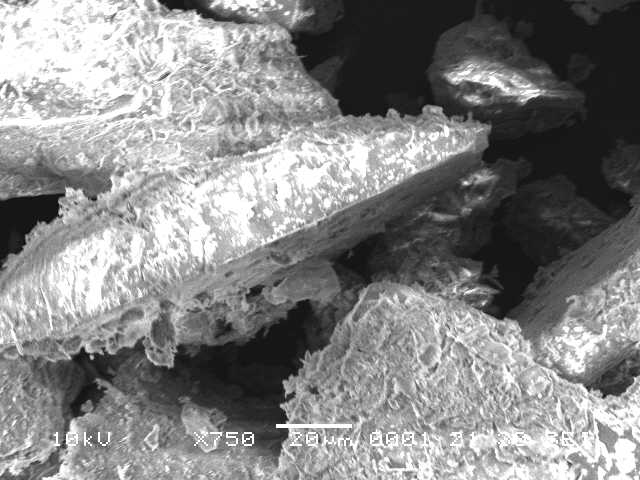
\includegraphics[width=\linewidth]{HKI_natural_azurite_x750_3_040521}
\end{minipage}
\caption[SEM images: Sample HKI, natural azurite]{SEM images: Sample HKI, natural azurite. Magnification: \textbf{left)} 250x, \textbf{right)} 750x.}
\label{fig:hki_nat_az_sem_1}
\end{figure}

\textit{Figure \ref{fig:hki_nat_az_sem_2}} shows images at 2000x and 4000x magnifications. At 2000x, sharp-sided and uneven particles are shown. At high magnification (4000x) significant size variation and interesting needle like crystal formations are observed. These appear to be orientated in some places, possibly showing the areas of crystal nucleation and growth. Other needle-like crystals are randomly orientated. This organisation is not  observed in other samples, though needle-like crystals are.

\begin{figure}[H]
\centering
\begin{minipage}{.45\textwidth}
  \centering
  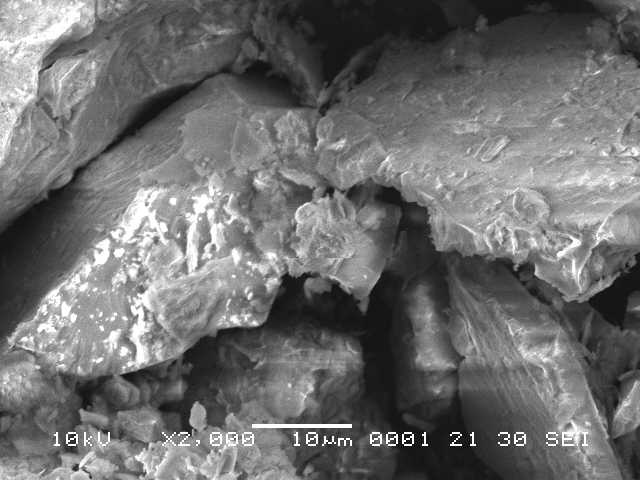
\includegraphics[width=\linewidth]{HKI_natural_azurite_x2000_3_040521}
\end{minipage}
\begin{minipage}{.45\textwidth}
  \centering
  \includegraphics[width=\linewidth]{HKI_natural_azurite_x4000_5_040521}
\end{minipage}
\caption[SEM images: Sample HKI natural azurite]{SEM images: Sample HKI natural azurite. Magnification: \textbf{left)} 2000x, \textbf{right)} 4000x.}
\label{fig:hki_nat_az_sem_2}
\end{figure}


% ************************************************     Az1     *******************************************************************

Sample Az1, likely from a natural source, is shown in \textit{Figure \ref{fig:az1_sem_1}} at 750x magnification (left) and 2000x magnification (right). The 750x image shows significant size variation. There are flat, sharp particles as well as many smaller particles. It is difficult to determine whether the larger pieces of sample are aggregates of smaller particles or larger intact pieces; the surfaces of these appear pocked.

At 2000x, the image shows the flat edge of a larger particle. Surface texture and grid formations are observed. These may be due to grinding and polishing of the pigment, but also may suggest some crystal ordering. Uniformity of shape and size is low at all magnifications and all over the sample.

\begin{figure}[H]
\centering
\begin{minipage}{.45\textwidth}
  \centering
  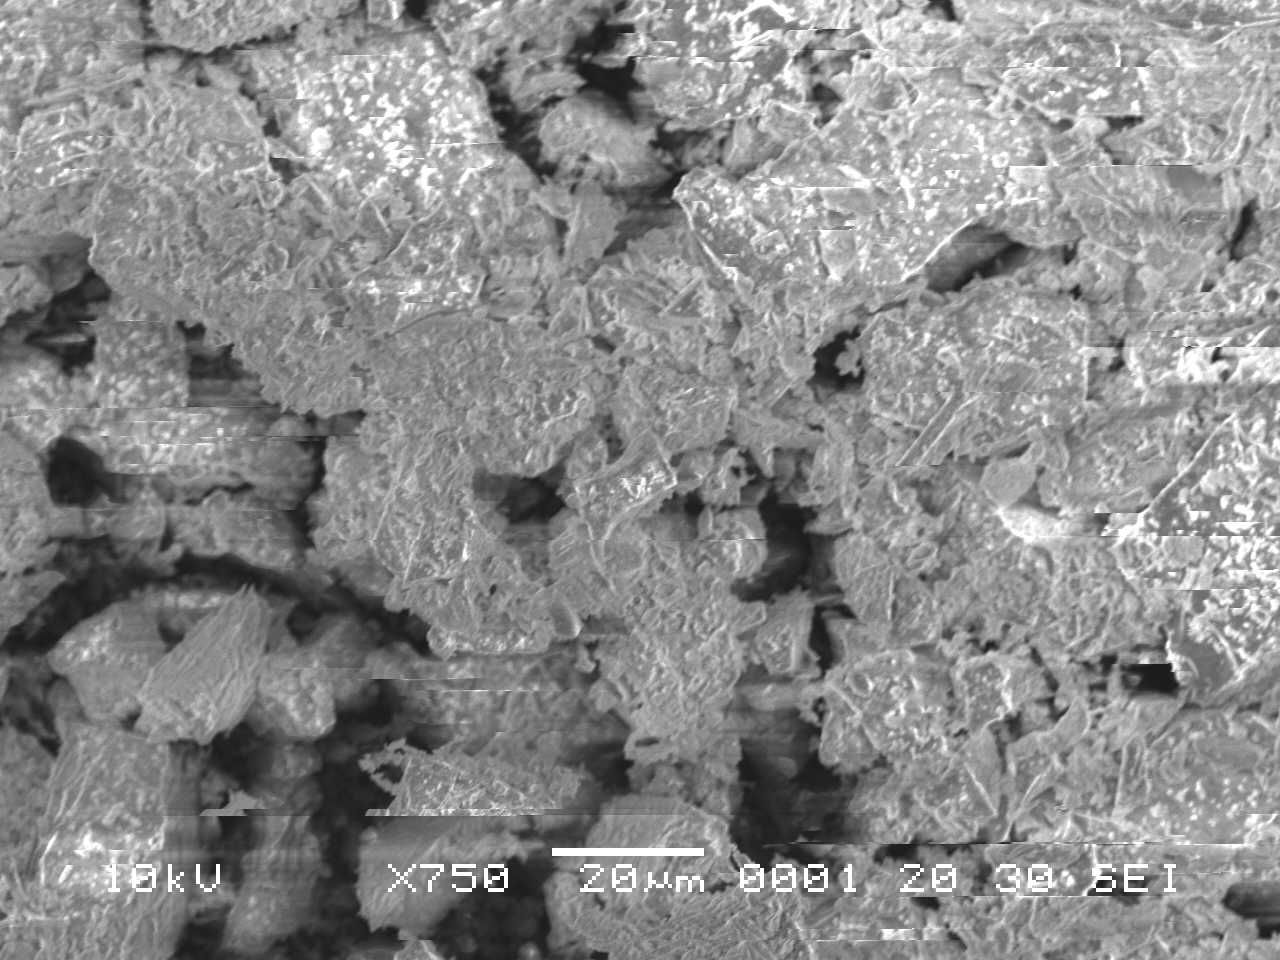
\includegraphics[width=\linewidth]{Az1_x750_3_220221}
\end{minipage}
\begin{minipage}{.45\textwidth}
  \centering
  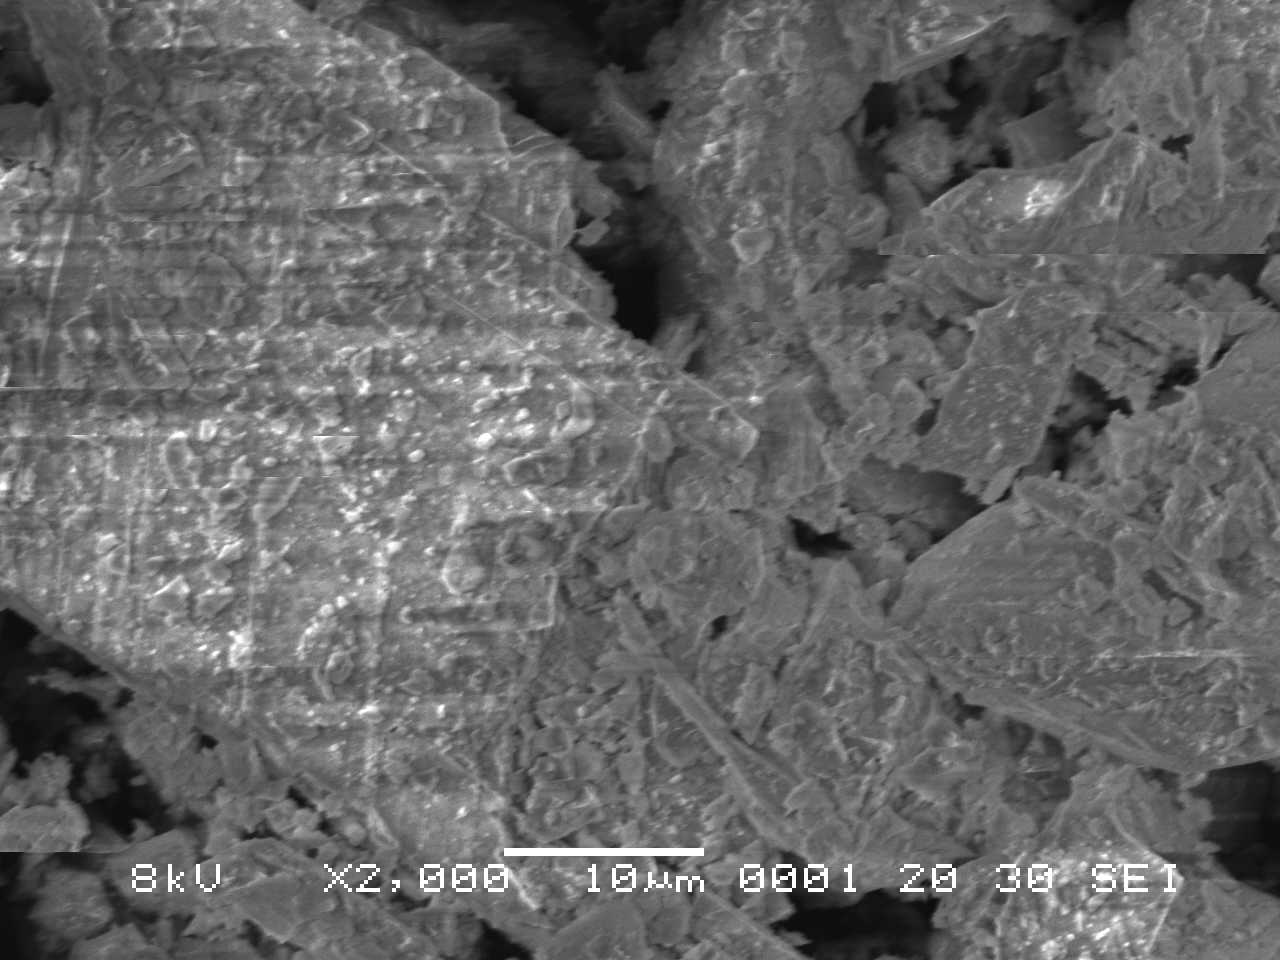
\includegraphics[width=\linewidth]{Az1_x2000_4_220221}
\end{minipage}
\caption[SEM images: Sample Az1, azurite]{SEM images: Sample Az1, azurite. Magnification: \textbf{left)} 750x, \textbf{right)} 2000x.}
\label{fig:az1_sem_1}
\end{figure}


% ************************************************     Az2     *******************************************************************

\textit{Figure \ref{fig:az2_sem_1}} shows sample Az2 at 200x and 1500x magnifications. Az2 is morphologically different from all other samples and lacks some features that appear to correlate with either natural or artificial pigment sources. Surface charging made it difficult to image, which was also not observed with most other samples.

It is interesting that although the shape of each particle is asymmetric and angular, the size and shape is quite consistent. At 200x magnification, the particle surfaces appear flat and smooth. These particles are much larger than the average size observed in other samples, which may suggest industrial pigment grinding. Otherwise, this consistency could also reflect a synthetic origin, with controlled conditions of crystal growth.

At 1500x magnification, there is minimal surface texture observed. Sample Az2 is unlike the sample HKI natural azurite. However, it also does not resemble known synthetic samples. Imaging at higher magnifications was not possible due to charging, though gold-coating the sample in the future may improve image quality.

\begin{figure}[H]
\centering
\begin{minipage}{.45\textwidth}
  \centering
  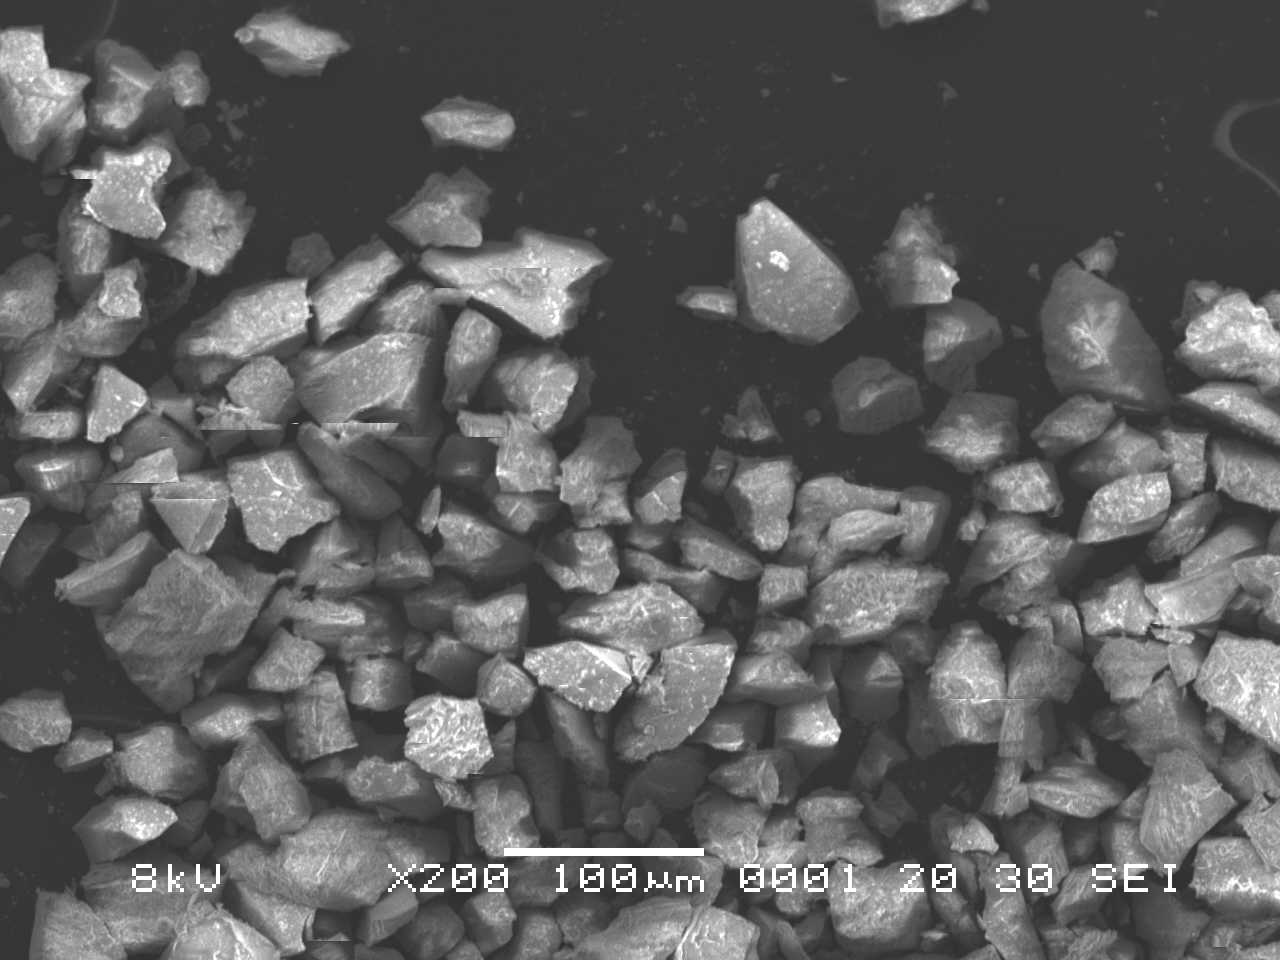
\includegraphics[width=\linewidth]{Az2_x200_1_240221}
\end{minipage}
\begin{minipage}{.45\textwidth}
  \centering
  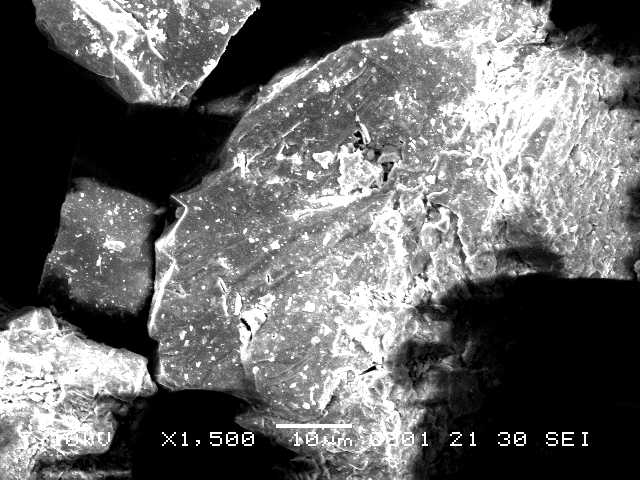
\includegraphics[width=\linewidth]{Az2_x1500_1_150321}
\end{minipage}
\caption[SEM images: Sample Az2, azurite]{SEM images: Sample Az2, azurite. Magnification: \textbf{left)} 200x, \textbf{right)} 1500x.}
\label{fig:az2_sem_1}
\end{figure}


% ************************************************     AzMag     *******************************************************************

\textit{Figure \ref{fig:azmag_sem_1}} show sample AzMag at 750x and 3000x magnifications. At 750x, the surfaces of particles are rough and highly textured. Most particles are approximately square or triangular, with a few small spheres on the surface. Elongated and large particles are not observed. The directionality observed in HKI natural azurite at high magnifications is not observed here. However, the degree of roughness and character of the surfaces is very similar, implying that this sample is naturally produced.

\begin{figure}[H]
\centering
\begin{minipage}{.45\textwidth}
  \centering
  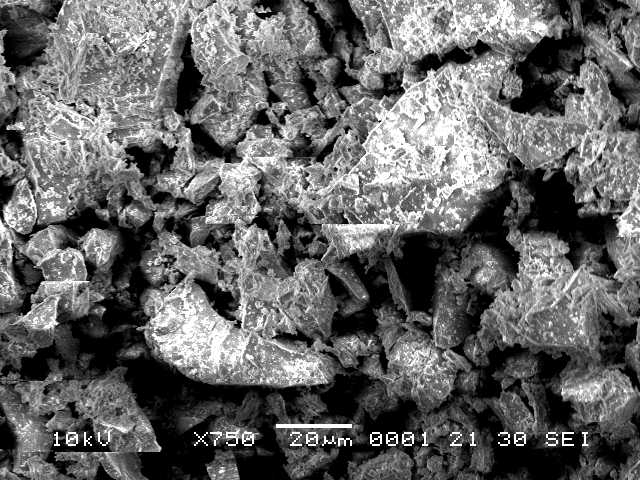
\includegraphics[width=\linewidth]{AzMag_x750_1_160321}
\end{minipage}
\begin{minipage}{.45\textwidth}
  \centering
  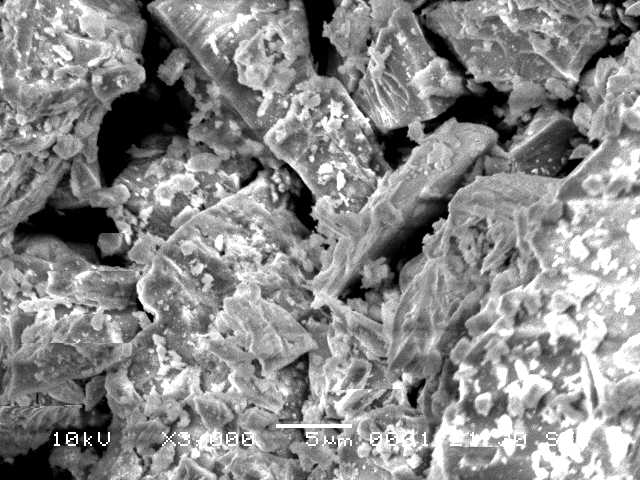
\includegraphics[width=\linewidth]{AzMag_x3000_1_160321}
\end{minipage}
\caption[SEM images: Sample AzMag, azurite]{SEM images: Sample AzMag, azurite. Magnification: \textbf{left)} 750x, \textbf{right)} 3000x.}
\label{fig:azmag_sem_1}
\end{figure}


% ************************************************     AzOp     *******************************************************************

\textit{Figures \ref{fig:azop_sem_1}} and \textit{\ref{fig:azop_sem_2}} show sample AzOp at 750x and 2000x magnifications. 

At 750x magnification (\textit{Figure \ref{fig:azop_sem_1}}, right), there are larger particles/aggregations present. It is difficult to tell whether these are single pieces or clumps of smaller particles. The shape of all particles is asymmetrical and varied, except in one specific case; at the bottom of the image there is a cluster of fairly uniformly spherical particles. 

\begin{figure}[H]
\centering
  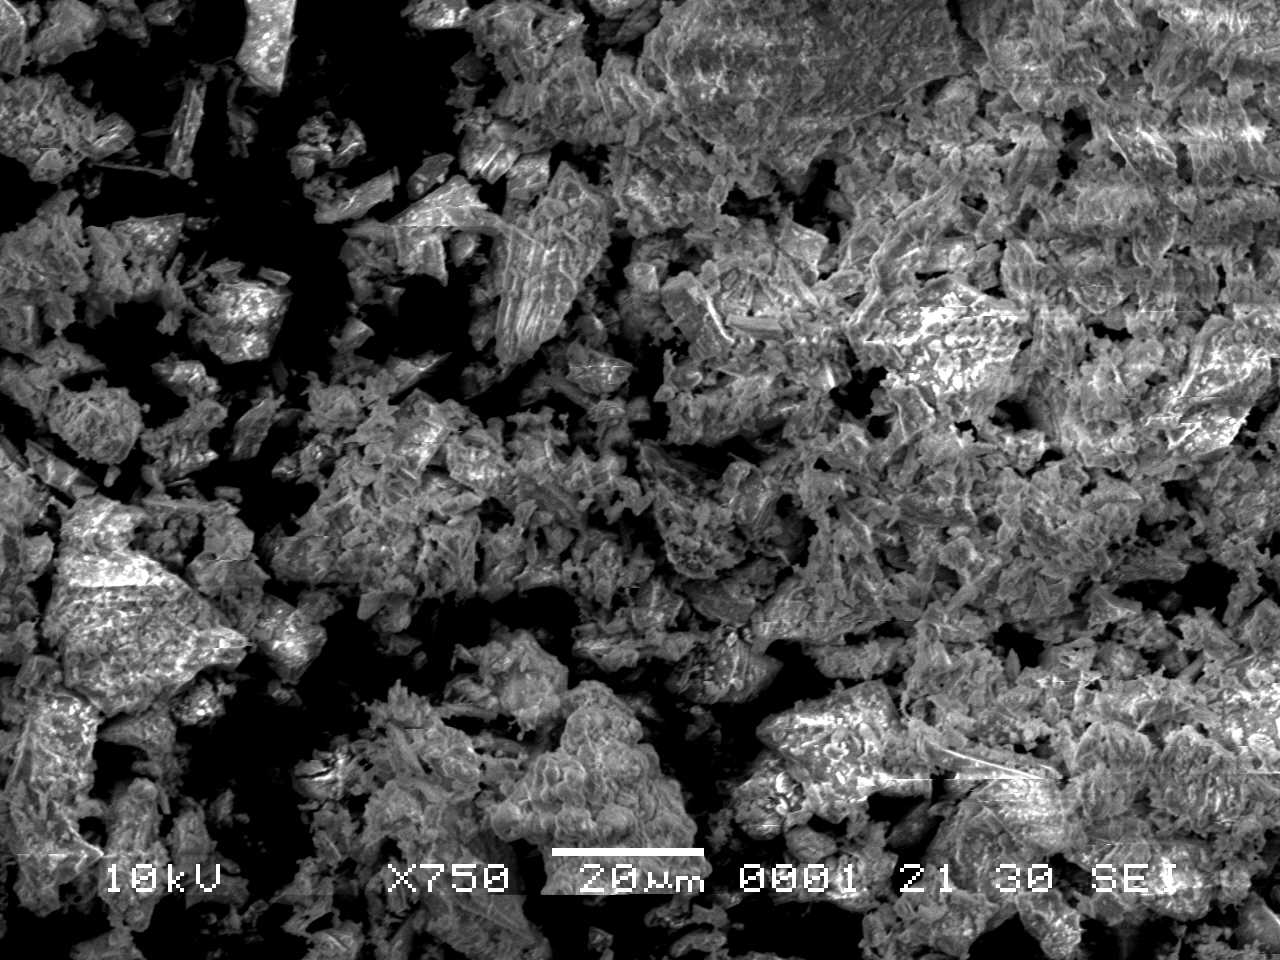
\includegraphics[width=.45\linewidth]{AzOp_x750_2_150321}
\caption[SEM image: Sample AzOp, azurite]{SEM image: Sample AzOp, azurite. Magnification: 750x.}
\label{fig:azop_sem_1}
\end{figure}

The spherical particles are clearly observed in \textit{Figure \ref{fig:azop_sem_2}}, right. They appear bubbly, as if many partial spheres have formed one on top of the other. This texture is not observed extensively in this sample, nor in other samples (e.g. AzMag, HKI natural azurite) that are broadly similar to AzOp. This could be the result of sample contamination, as several samples were analysed at the same time, or this could be evidence of multiple conditions under which crystals formed before being mixed to make this pigment. This type of morphology is uniform and does not look like the result of random crushing and grinding. This should be investigated further by imaging over a larger area of this sample and by preparing additional fresh samples. Sample preparation may also bias samples to contain more particles of a particular size due to separation in storage.

In contrast, the rougher and more heterogeneous texture of the majority of the sample is shown at 2000x magnification in \textit{Figure \ref{fig:azop_sem_2}}, left. Few circular particles are seen, and size and shape very. This is very similar to natural samples.

\begin{figure}[H]
\centering
\begin{minipage}{.45\textwidth}
  \centering
  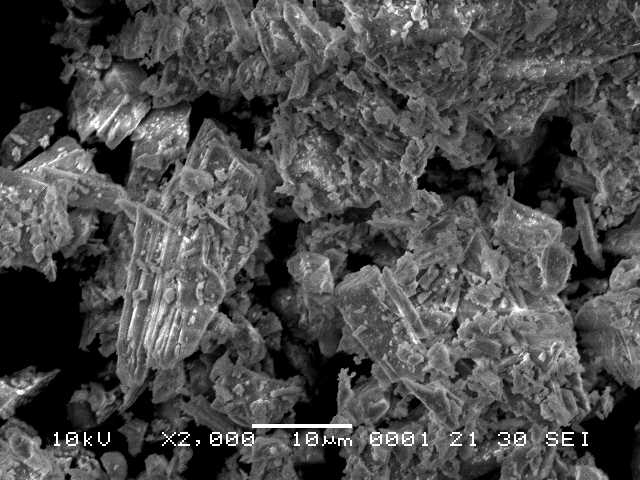
\includegraphics[width=\linewidth]{AzOp_x2000_1_150321}
\end{minipage}
\begin{minipage}{.45\textwidth}
  \centering
  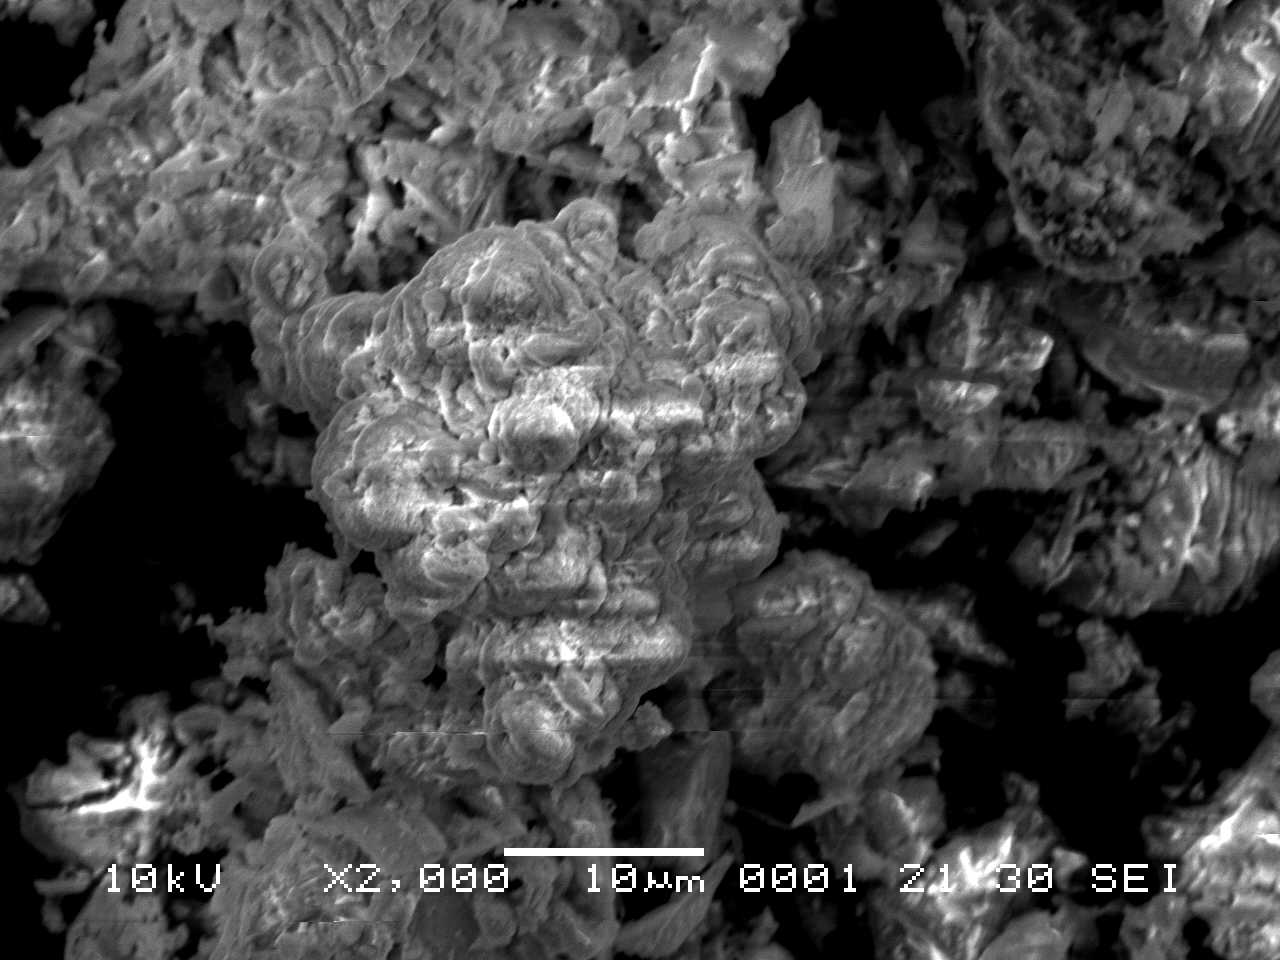
\includegraphics[width=\linewidth]{AzOp_x2000_4_150321}
\end{minipage}
\caption[SEM images: Sample AzOp, azurite]{SEM images: Sample AzOp, azurite. Magnification: 2000x}
\label{fig:azop_sem_2}
\end{figure}

% ************************************************     Fitz1     *******************************************************************
\textit{Figure \ref{fig:Fitz1_sem_1}} shows sample Fitz1 at 750x and 1500x magnifications. This sample is blue verditer, and a commercial product number is provided allowing confirmation that this is a synthetic product.

At 750x magnification (\textit{Figure \ref{fig:Fitz1_sem_1}}, left), it is possible to qualitatively assess the diameter of particles as consistently < 5 $\mu$m. Particles resemble the spherical cluster observed in the sample AzOp. Size and shape are both regular, but it is difficult to determine whether the particles are flat discs or stacked semicircles occupying more volume.

At 1500x magnification (\textit{Figure \ref{fig:Fitz1_sem_1}}, right), there are clearly spherical particles. These have aggregated. The size is similar to the spherical cluster in the AzOp sample. The surface also looks slightly pocked or porous. 

\begin{figure}[H]
\centering
\begin{minipage}{.45\textwidth}
  \centering
  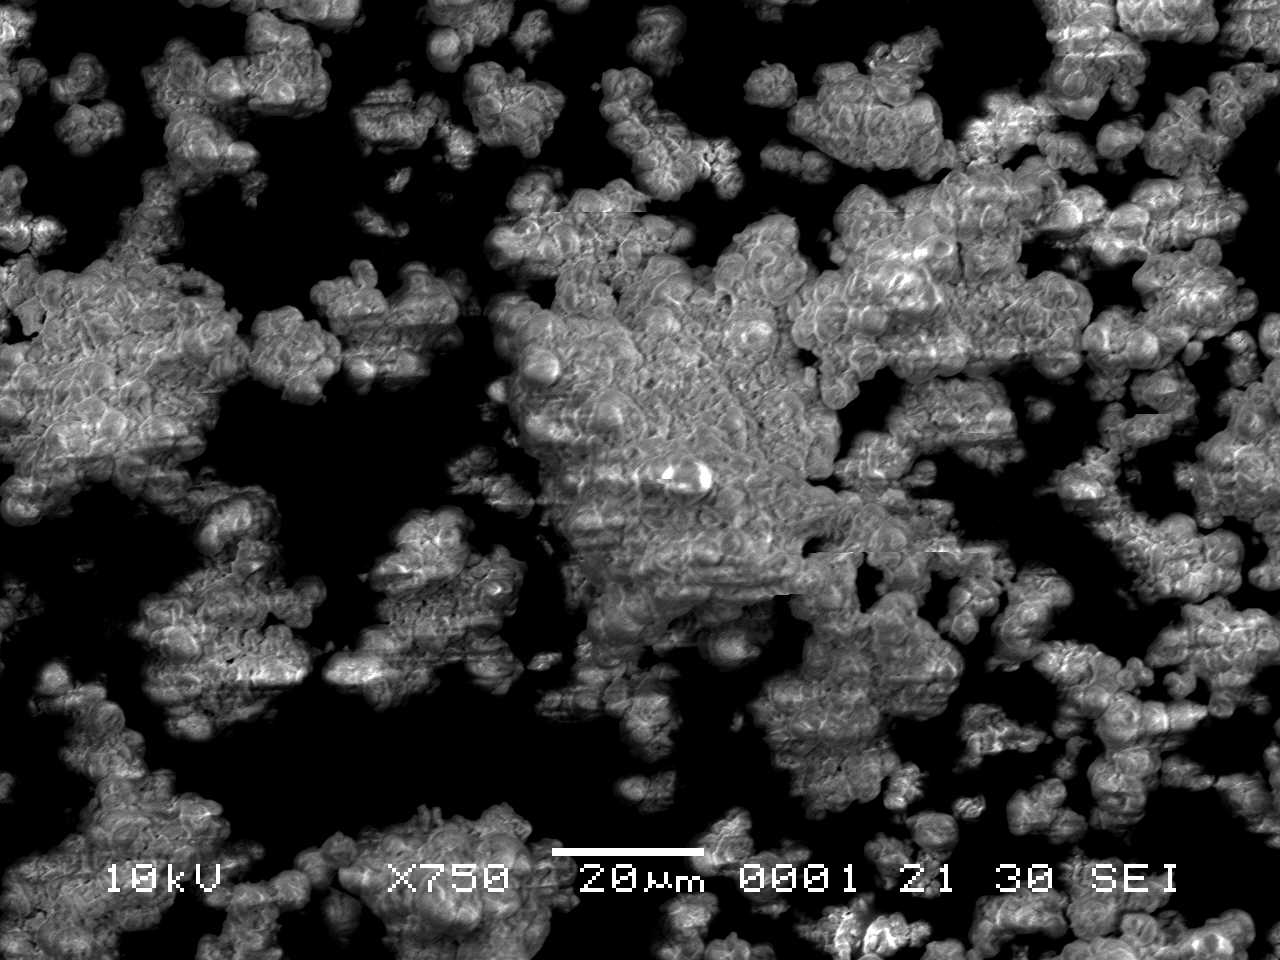
\includegraphics[width=\linewidth]{Fitz1_x750_1_030321}
\end{minipage}
\begin{minipage}{.45\textwidth}
  \centering
  \includegraphics[width=\linewidth]{Fitz1_x1500_2_030321}
\end{minipage}
\caption[SEM images: Sample Fitz1, blue verditer]{SEM images: Sample Fitz1, blue verditer. Magnification: \textbf{left)} 750x, \textbf{right)} 1500x}
\label{fig:Fitz1_sem_1}
\end{figure}


% ************************************************     KE3     *******************************************************************

\textit{Figure \ref{fig:KE3_sem_1}} shows sample KE3 at 750x and 2000x magnifications. KE3 is described as light verditer bice. Verditer suggests a synthetic origin, while bice is used to refer to both natural and synthetic blue pigments. Tentatively, this sample is interpreted to be synthetic based on this information.

At 750x magnification (\textit{Figure \ref{fig:KE3_sem_1}}, left), particle uniformity is apparent. They are symmetric and spherical, but more angular than sample Fitz1. There are areas of needle-like structures and stacks of spherical or octagonal particles forming small aggregates. At 2000x magnification (\textit{Figure \ref{fig:KE3_sem_1}}, right), spheres are observed. There is significant texture on the surface that is quite fine especially around the edges of particles, and this texture appears rougher than that of sample Fitz1. The approximate particle size can be approximated to 5-10 $\mu$m.

\begin{figure}[H]
\centering
\begin{minipage}{.45\textwidth}
  \centering
  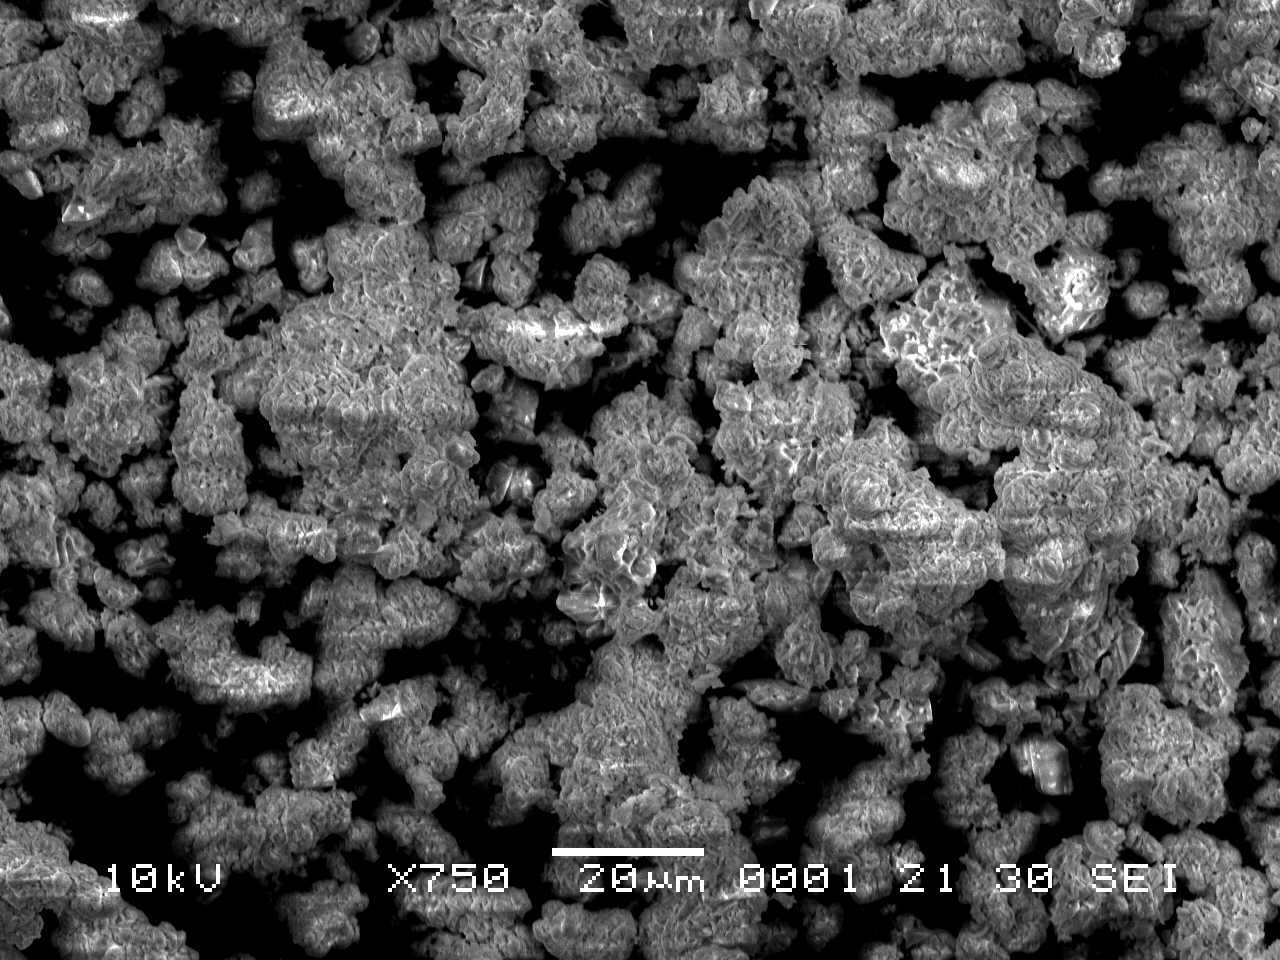
\includegraphics[width=\linewidth]{KE3_x750_3_050321}
\end{minipage}
\begin{minipage}{.45\textwidth}
  \centering
  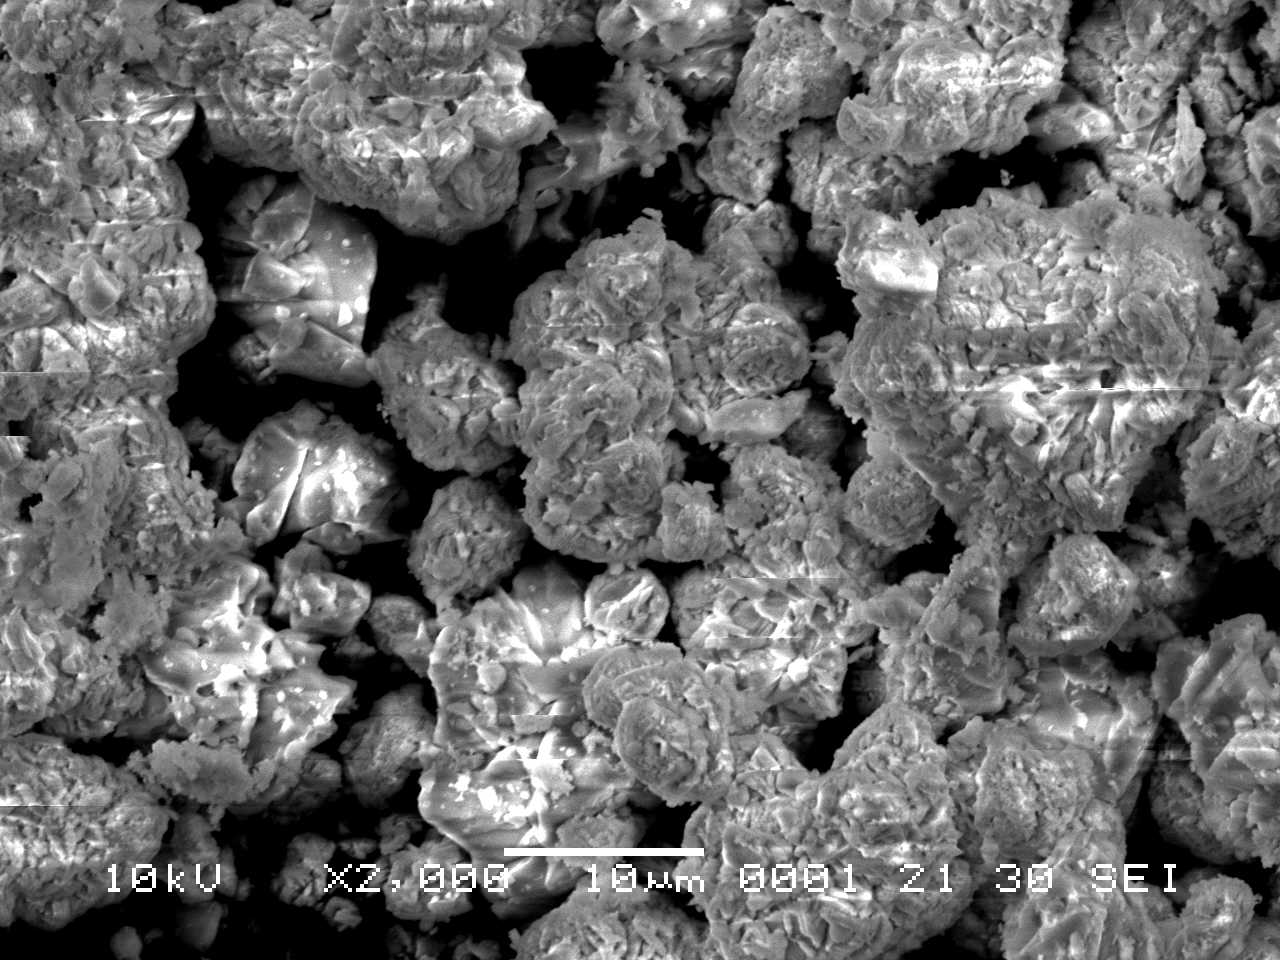
\includegraphics[width=\linewidth]{KE3_x2000_2_050321}
\end{minipage}
\caption[SEM images: Sample KE3, light verditer bice]{SEM images: Sample KE3, light verditer bice. Magnification: \textbf{left)} 750x, \textbf{right)} 2000x}
\label{fig:KE3_sem_1}
\end{figure}

% ************************************************     KE4     *******************************************************************

\textit{Figure \ref{fig:KE4_sem_1}} shows sample KE4 at magnifications at 750x and 2000x. KE4 is labelled as blue bice, which is an ambiguous description, so its origin is inconclusive.

At 750x magnification (\textit{Figure \ref{fig:KE4_sem_1}}, left), fine needle-like structure is visible, similar to sample HKI natural azurite. There are also rounder structures that resemble Fitz1. Larger particles on the order of 50 $\mu$m are visible, as are smaller particles on the order of 5 $\mu$m. \textit{Figure \ref{fig:KE4_sem_1}} (right) shows KE4 at 2000x magnification. The image shows the flat side of a larger particle (or aggregate) with smaller particles attached to or resting on the surface. There are also cavities observed. This sample shows characteristics of known natural as well as synthetic samples.

\begin{figure}[H]
\centering
\begin{minipage}{.45\textwidth}
  \centering
  \includegraphics[width=\linewidth]{KE4_x750_1_030321}
\end{minipage}
\begin{minipage}{.45\textwidth}
  \centering
  \includegraphics[width=\linewidth]{KE4_x2000_1_030321}
\end{minipage}
\caption[SEM images: Sample KE4, blue bice]{SEM images: Sample KE4, blue bice. Magnification: \textbf{left)} 750x, \textbf{right)} 2000x}
\label{fig:KE4_sem_1}
\end{figure}


% ************************************************     KE5     *******************************************************************

\textit{Figure \ref{fig:KE5_sem_1}} shows sample KE5 at 750x and 1500x magnifications. KE5 is described as blue verditer, strongly suggesting a synthetic origin.

At 750x magnification, larger aggregates of approximately 80 $\mu$m are clearly seen to be formed from smaller particles, similar to Fitz1. Particles appear to be intersecting flat discs forming circular or semicircular three dimensional structures. \textit{Figure \ref{fig:KE5_sem_1}} (right) shows KE5 at 1500x magnification. The circular character of particles is clearly observed.

%~\autocite{hope_gypsum}

\begin{figure}[H]
\centering
\begin{minipage}{.45\textwidth}
  \centering
  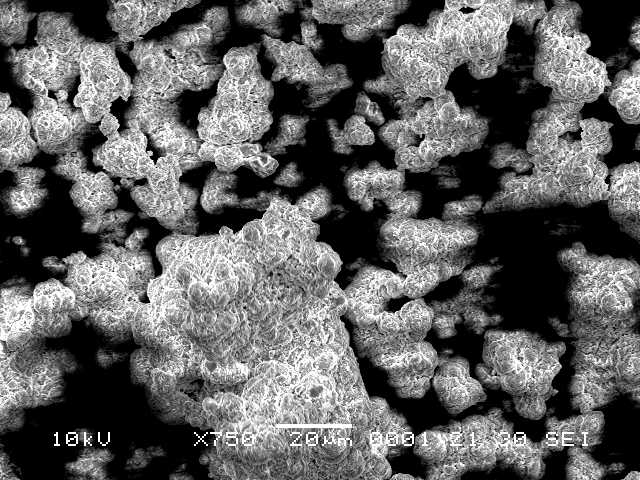
\includegraphics[width=\linewidth]{KE5_x750_1_050321}
\end{minipage}
\begin{minipage}{.45\textwidth}
  \centering
  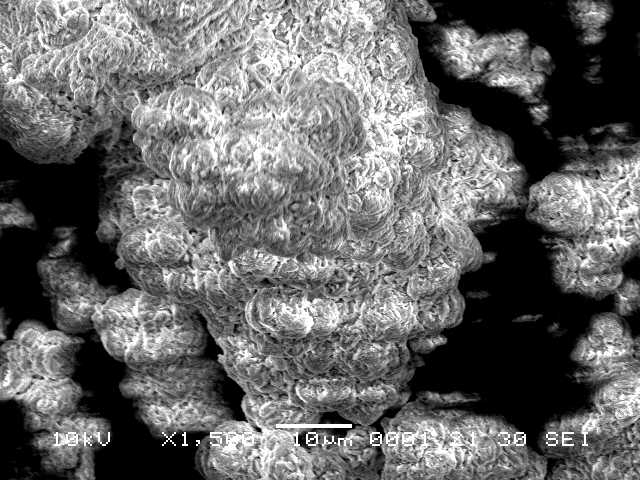
\includegraphics[width=\linewidth]{KE5_x1500_1_050321}
\end{minipage}
\caption[SEM images: Sample KE5, blue verditer]{SEM images: Sample KE5, blue verditer. Magnification: \textbf{left)} 750x, \textbf{right)} 1500x}
\label{fig:KE5_sem_1}
\end{figure}

\subsubsection[Particle size distribution of natural and artificial azurite]{Particle size distribution of natural and artificial azurite}
\label{subsubsection3.1.1.1}

SEM images at 750x magnification of loosely dispersed particles were collected. The two powder samples, HKI natural azurite and Fitz1, were selected based on their known sources and varied morphology. The cross section was also analysed. The cross section was also analysed using the same method. These images were processed in ImageJ (Version 1.53a) by increasing contrast and manually thresholding followed by manual selection of maximum lengths and measurement.

Five images of Fitz1 were analysed, with n(particles) = 102. Five images of HKI natural azurite were analysed, with n(particles) = 127. Three images of the cross section were analysed, with n(particles) = 153. There is undoubtedly some bias in selected particles due to the difficulty of defining edges in the images, and this may affect the spread of results. An example of the original SEM image (left) and the thresholded binary image (right, used for measurements) is shown for sample Fitz1 in \textit{Figure \ref{fig:imageJ_fitz1}}.

\begin{figure}[H]
\centering
\begin{minipage}{.45\textwidth}
  \centering
  \includegraphics[width=\linewidth]{Fitz1_x750_5_130521}
\end{minipage}
\begin{minipage}{.45\textwidth}
  \centering
  \includegraphics[width=\linewidth]{Fitz1_x750_5_130521_BW}
\end{minipage}
\caption[Particle size analysis: Sample Fitz1]{Particle size analysis: Sample Fitz1. \textbf{Left)} original SEM image, \textbf{Right)} thresholded binary image.}
\label{fig:imageJ_fitz1}
\end{figure}

Measurements from each image were combined and analysed using RStudio (Version 1.3.1093) to produce a histogram of the frequency of length measurements (bin size = 1 $\mu$m), shown in \textit{Figure \ref{fig:histogram_length}}. Based on the different particle morphologies, it would be reasonable to expect that the particle size distribution would differ between samples. Additionally, the presence of a bimodal distribution in the histogram might indicate the formation of aggregates of a specific size. 

The length distributions of Fitz1 and HKI natural azurite do not differ significantly. Both show peak lengths around 5 $\mu$m, with a low frequency of particles or clusters above 10 $\mu$m. Sample Fitz1 does show several particles of length around 15 $\mu$m, which is absent in HKI natural azurite. This could suggest that aggregates form at more consistent sizes in Fitz1. Overall, these two samples are statistically very similar. \textit{Table \ref{table:r_stats}} summarises statistics, and it is notable how similar the means (and to some extent medians) are. There is a wider range of particle lengths in the natural azurite sample, though this may be due to processing since the cross section shows overall smaller particle sizes than both powder samples. 

This analysis is expanded in Chapter 4 to include a larger sample size and analysis of the skew of particle shapes. While this initial work established the feasibility and utility of particle size analysis, a larger sample size should be used to study both Fitz1 and HKI natural azurite to draw statistically sound conclusions, and a discussion of particle skew should be added.

\begin{figure}[H]
\centering
\begin{minipage}{.45\textwidth}
  \centering
  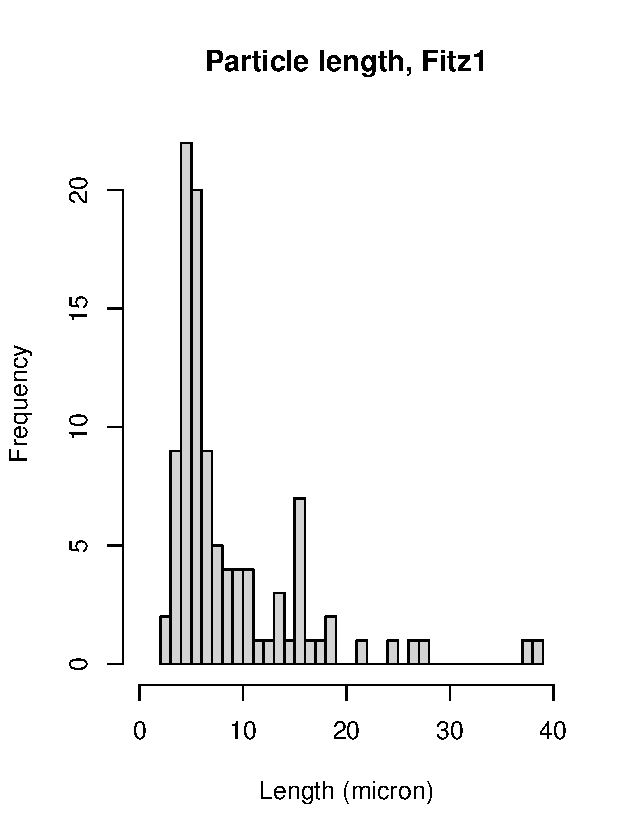
\includegraphics[width=\linewidth]{hist_fitz1}
\end{minipage}
\begin{minipage}{.45\textwidth}
  \centering
  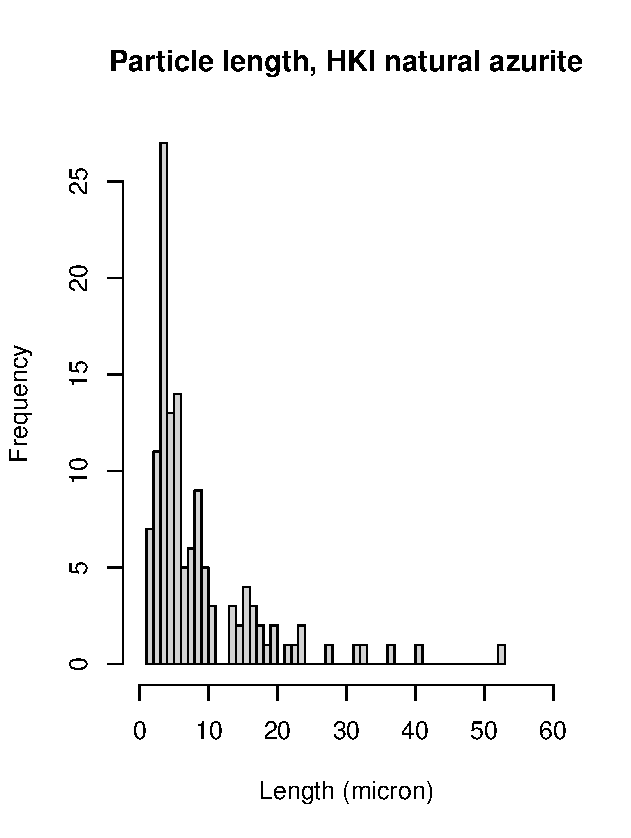
\includegraphics[width=\linewidth]{hist_hki}
\end{minipage}
\caption[Particle size analysis: HKI natural azurite, Fitz1]{Particle size analysis: Sample HKI natural azurite. \textbf{Left)} Fitz1, \textbf{Right)} HKI natural azurite.}
\label{fig:histogram_length}
\end{figure}

\begin{figure}[H]
\centering
  \includegraphics[width=0.45\linewidth]{hist_xsection}
\caption[Particle size analysis: cross section]{Particle size analysis: cross section.} 
\label{fig:hist_xsec}
\end{figure}

\begin{table}[H]
\caption{Descriptive statistics: Fitz1, HKI natural azurite, cross section}
\centering
\label{table:r_stats}
\begin{tabular}{c c c c}
\toprule
Reference sample & Mean & Median & Range \\
\midrule
HKI natural azurite & 8.583 & 5.437 & 1.177 - 52.176 \\
Fitz1 & 8.683 & 5.878 & 2.414 - 38.367 \\
Cross section & 8.328 & 7.648 & 2.142 - 28.930 \\
\bottomrule
\end{tabular}
\end{table}

The three samples are compared side-by-side in \textit{Figure \ref{fig:hist_all}}. The effect of outliers on the mean values of particle sizes is apparent, since both powder samples (black, red) show length distributions that, apart from a few larger outliers, are located at smaller lengths than that of the cross section in spite of all three datasets having very similar mean values. 

The difference between the powder samples and the cross section may be due to a number of factors. The preparation of pigments likely differed in the 15th century compared to today, though since azurite's optical properties depend on the size of its particle grains, we expect the fineness of grinding not to vary wildly. 

Suspension in a binding medium may affect the dispersion of grains, and this could affect aggregation (whether or not it would hinder aggregation depends on the hydrophilicity of the mineral, which is low in the case of azurite).~\autocite{Zhang} Optimal dispersion may also be orientation dependent. Sampling bias will be present as only the x and y dimensions of the grains can be measured using this method, and depending on the orientation of particles relative to the slicing of the cross section, certain orientations may be over or underrepresented. 

The preparation of the cross section by resin embedding followed by microtoming will affect the appearance of particles under SEM. Microtoming may visually flatten the particles, making it difficult to see smaller grains. 

\begin{figure}[H]
\centering
  \includegraphics[width=0.9\linewidth]{hist_fitz1_hki_xsec_largerange_edit}
\caption[Particle size analysis: HKI natural azurite, Fitz1, cross section]{Particle size analysis: Fitz1 (black), HKI natural azurite (red), cross section (blue).} 
\label{fig:hist_all}
\end{figure}


%fitz1
%Median : 5.878  
%Mean   : 8.683
%range 2.414 to 38.367
% hki 
%Median : 5.437  
%Mean   : 8.583
%range 1.177 to 52.176

% *******************************************************************************************************************************
% *******************************************************************************************************************************
% *******************************************************************************************************************************

\subsection[Malachite and green verditer]{Malachite and green verditer}
\label{subsection3.1.2}

% ************************************************     Ma1     *******************************************************************

\textit{Figures \ref{fig:Ma1_sem_1}} and \textit{\ref{fig:Ma1_sem_2}} show sample Ma1 at magnifications from 750x to 3000x. This sample is natural malachite. At 750x magnification, particles appear highly irregular. They have rough and choppy edges, and their irregular shapes closely resemble those of natural azurite samples. Few aggregates are larger than 20 $\mu$m. At high magnification, the sample is disordered and heterogeneous. Many particles under 1 $\mu$m across are present, with extremely uneven borders. These are unambiguously single particles rather than surface roughness.

\begin{figure}[H]
\centering
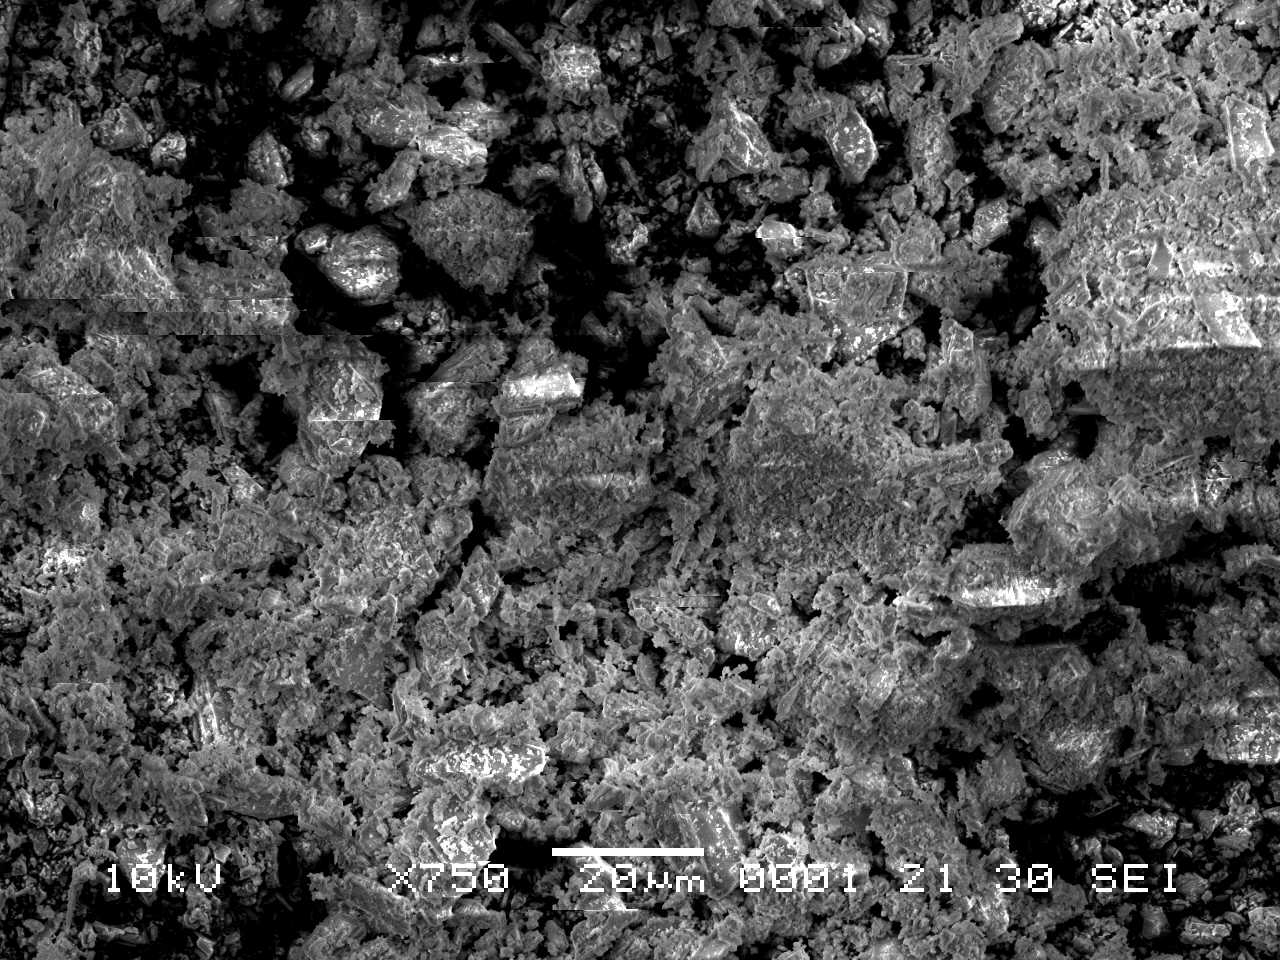
\includegraphics[width=0.45\linewidth]{Ma1_x750_2_160321}
\caption[SEM images: Sample Ma1, malachite]{SEM images: Sample Ma1, malachite. Magnification: 750x.}
\label{fig:Ma1_sem_1}
\end{figure}

\begin{figure}[H]
\centering
\begin{minipage}{.45\textwidth}
  \centering
  \includegraphics[width=\linewidth]{Ma1_x2500_3_160321}
\end{minipage}
\begin{minipage}{.45\textwidth}
  \centering
  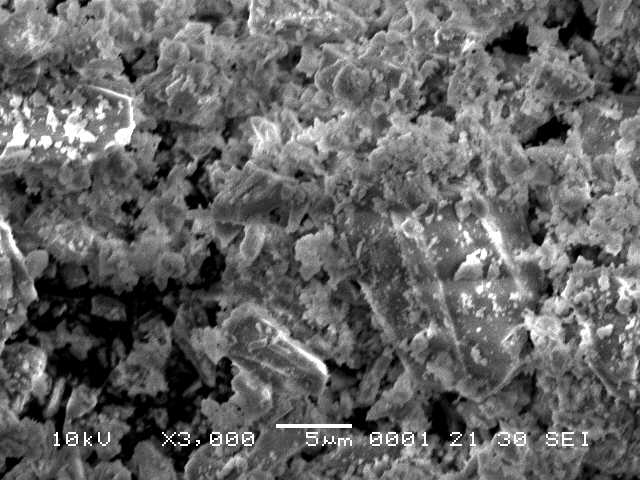
\includegraphics[width=\linewidth]{Ma1_x3000_2_160321}
\end{minipage}
\caption[SEM images: Sample Ma1, malachite]{SEM images: Sample Ma1, malachite. Magnification: \textbf{left)} 2500x, \textbf{right)} 3000x.}
\label{fig:Ma1_sem_2}
\end{figure}

% ************************************************     KE1a     *******************************************************************

\textit{Figure \ref{fig:KE1a_sem_1}} shows sample KE1a at magnifications 250x (left) and 750x (right). The name of KE1a, green bice, is ambiguous.

At 250x magnification, small particles form aggregations of approximately 25-50 $\mu$m. The shapes of particles appear to be squared-off circles with some degree of uniformity. They are not, however, spherical like several verditer samples discussed above. 

This sample is more uniform and spherical than sample Ma1 but it is more challenging to draw clear conclusions about morphological differences between natural and synthetic green samples compared to blue. There is a much smaller sample size in the reference samples available, as well as ambiguity in sample source. However, this also may suggest that green samples do not show marked morphology differences depending on origin.

\begin{figure}[H]
\centering
\begin{minipage}{.45\textwidth}
  \centering
  \includegraphics[width=\linewidth]{KE1a_x250_1_040321}
\end{minipage}
\begin{minipage}{.45\textwidth}
  \centering
  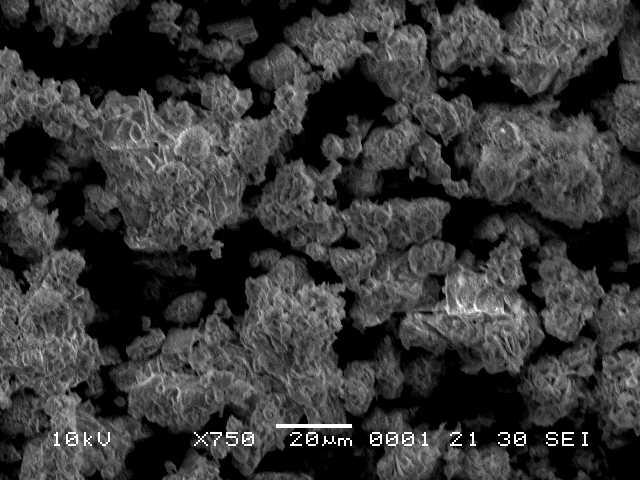
\includegraphics[width=\linewidth]{KE1a_x750_2_040321}
\end{minipage}
\caption[SEM images: Sample KE1a, green bice]{SEM images: Sample KE1a, green bice. Magnification: \textbf{left)} 250x, \textbf{right)} 750x}
\label{fig:KE1a_sem_1}
\end{figure}

% ************************************************     KE1b     *******************************************************************

%didnt do this one

% ************************************************     KE2     *******************************************************************

\textit{Figure \ref{fig:KE2_sem_1}} shows sample KE2, green verditer, at 750x (left) and 2000x (right) magnifications. The sample name implies synthetic origin. 

At 750x magnification, particles are irregular, sharp, and not elongated. At 2000x magnification, there is a lack of texture on the surface of individual particles. The edges of particles are feathery, which is observed in other samples as well. It is possible to estimate the particle size at approximately 7-10 $\mu$m. 

\begin{figure}[H]
\centering
\begin{minipage}{.45\textwidth}
  \centering
  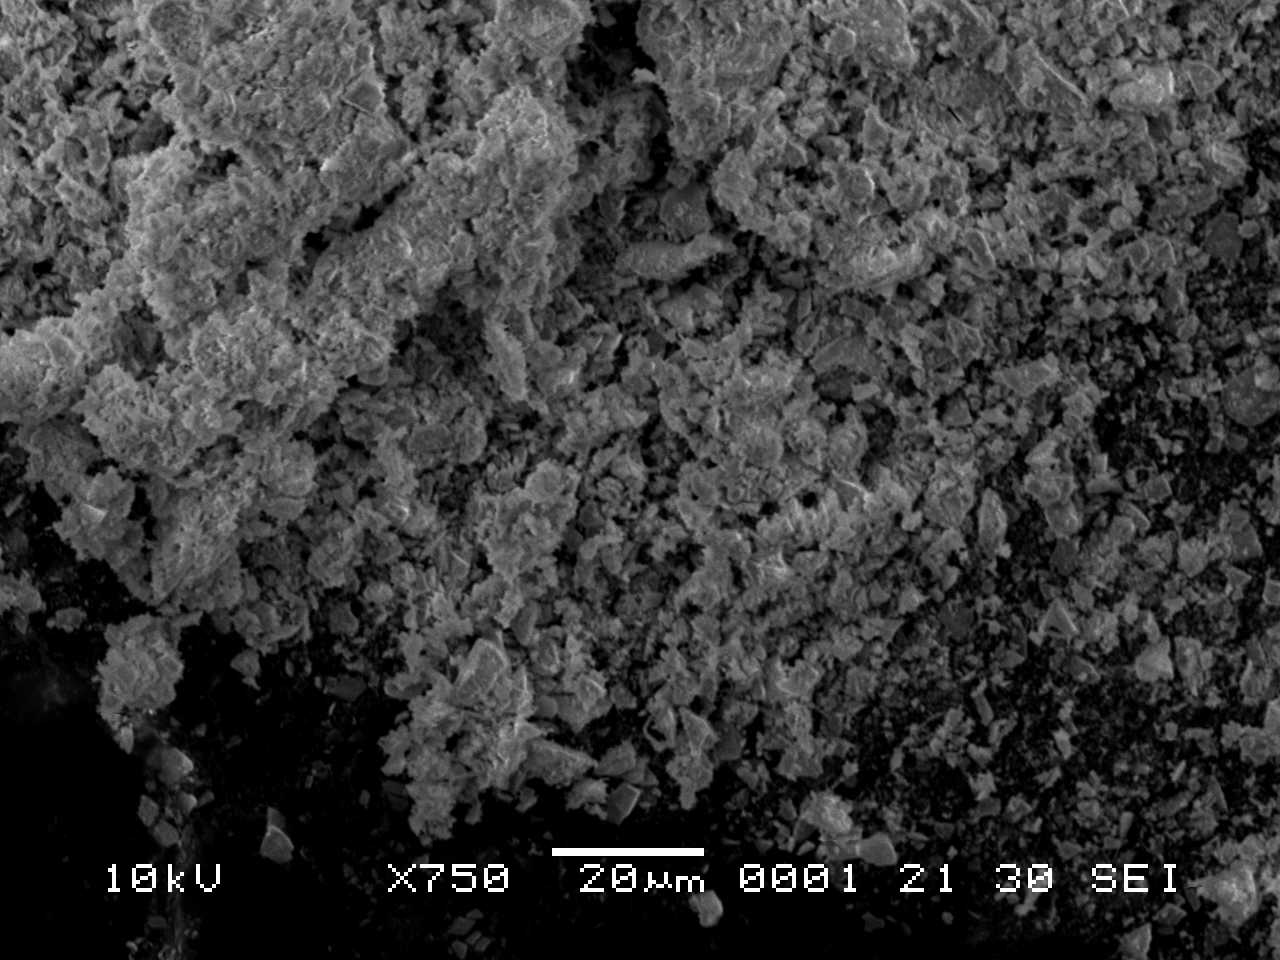
\includegraphics[width=\linewidth]{KE2_x750_1_040321}
\end{minipage}
\begin{minipage}{.45\textwidth}
  \centering
  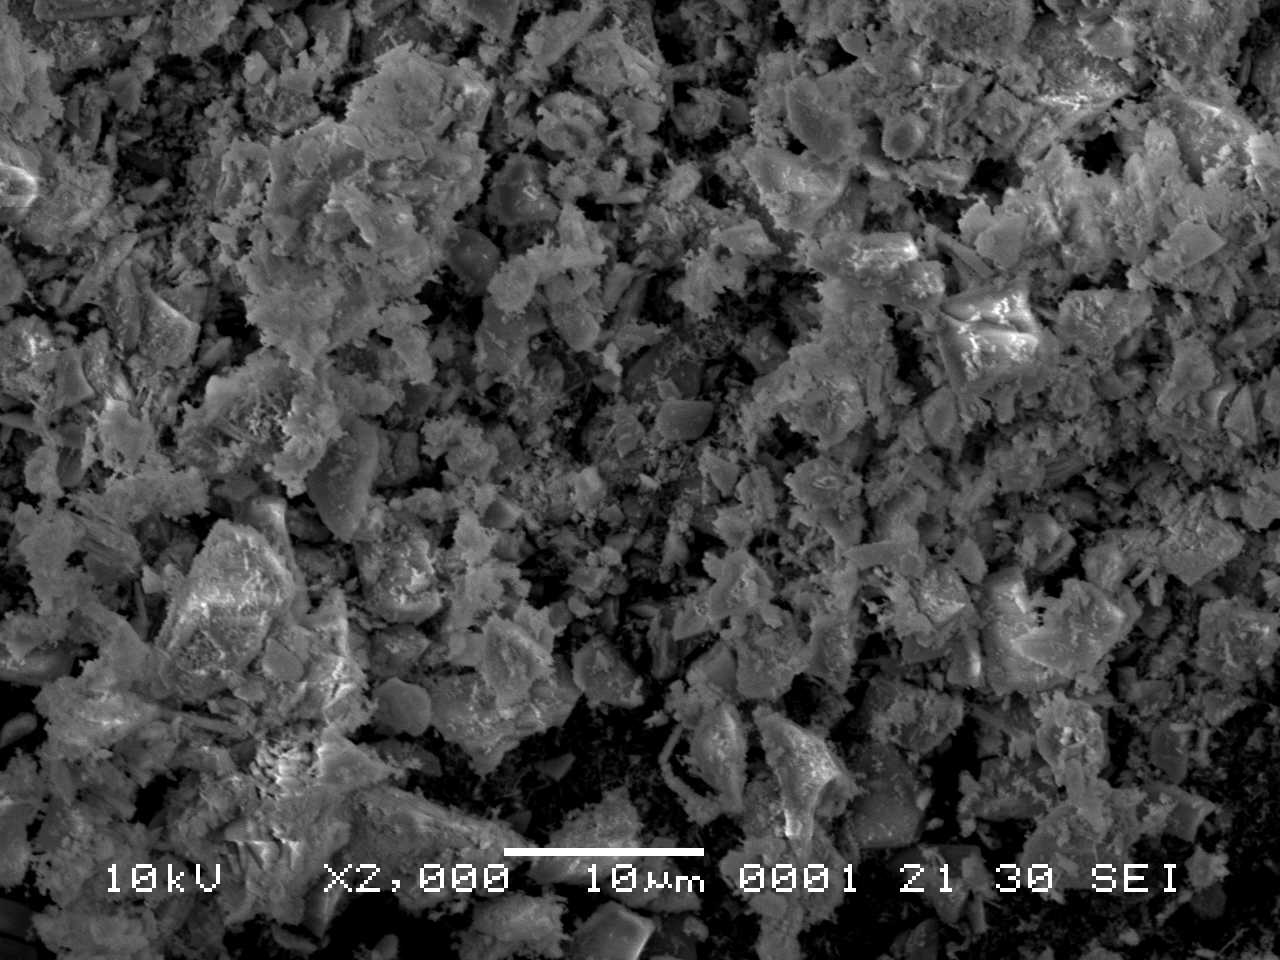
\includegraphics[width=\linewidth]{Ke2_x2000_1_040321}
\end{minipage}
\caption[SEM images: Sample KE2, green verditer]{SEM images: Sample KE2, green verditer. Magnification: \textbf{left)} 750x, \textbf{right)} 2000x}
\label{fig:KE2_sem_1}
\end{figure}


\subsection[Historical samples]{Historical samples}
\label{subsection3.1.3}

SEM images of a cross section removed from a 16th c. old masters work (\textit{Birth of Jupiter}, Giulio Romano, azurite/verditer layers c. 1530 and 1630) are presented.

Images were collected on two different instruments, a JEOL JSM-5510LV SEM (coupled with an Oxford Instruments INCA EDS system) and a TESCAN MIRA3 FEG-SEM (coupled with an Oxford Instruments Aztec Energy X-maxN 80 EDS system). The sample was coated with 24 nm carbon. On the JEOl SEM, images were collected using the backscatter electron detector (BES) which is sensitive to atomic weight: heavier elements appear lighter in BES images. The BES detector was used in low vacuum mode. On the TESCAN SEM, images were collected using the secondary electron detector (SE) and the BES detector simultaneously. 

\textit{Figure \ref{fig:xsection_jeol_1}} (left) shows the cross section at low magnification (750x, JEOl). Three distinct layers are visible. The sample contains natural azurite and artificial blue verditer pigment particles, as well as other pigments and some form of organic binder in which the pigment particles are embedded. Thin cracks divide the layers and the entire cross section vertically. \textit{Figure \ref{fig:hki_crossec_explanation}} labels these three layers A, B, C, with C containing lower atomic weight components. 

The size and shape of pigment particles is uneven. The medium grey pigment in layers A and B is copper-based according to EDS. EDS also allow assignment of the bright white particles to lead, likely lead carbonate based on presence of oxygen, absence of chromium/tin (components of lead yellow), and the cross section colour. The copper based particles are morphologically distinct from the lead and manganese (darkest) particles, with dimensions on the order of 10-20 $\mu$m.

\textit{Figures \ref{fig:xsection_jeol_1}} (right) and \textit{\ref{fig:xsection_jeol_2}} show the cross section at high magnification (1400-2500x, JEOL), and \textit{Figures \ref{fig:xsection_dept_1}} and \textit{\ref{fig:xsection_dept_2}} show the cross section at 4300x and 12,500x magnification (TESCAN instrument). The JEOl instrument in BES shows much more apparent contrast between different elements than the TESCAN instrument, making it more straightforward to interpret. The TESCAN instrument, on the other hand, shows both BES (left) and SE (right) images and shows overall structure but does not clearly distinguish between pigments visually. Pitting and cracks are visible. One feature that is not easily explained is the feathery, indistinctly bound areas of white in the BES images. As this feature is not present in the SE images, it is not explained by surface charging. Morphologically, it looks to be due to an organic binder or embedding resin.

At higher magnification, the irregularity of orientation and shape of particles is clear. \textit{Figure \ref{fig:xsection_dept_2}} shows the sample at high magnification in an area where copper blue pigments are expected to be present. Interesting planar morphology is shown, resembling Az1 and AzMag.

\begin{figure}[H]
\centering
  \includegraphics[width=0.6\linewidth]{hki_crossec_explanation}
\caption[Cross section with visually distinct layers A, B, and C labelled]{Cross section, SEM image at 550x magnification, with visually distinct layers A, B, and C labelled.}
\label{fig:hki_crossec_explanation}
\end{figure}

\begin{figure}[H]
\centering
\begin{minipage}{.45\textwidth}
  \centering
  \includegraphics[width=\linewidth]{hki_xsection_BES_LV_x750_2_58spot_240621}     
\end{minipage}
\begin{minipage}{.45\textwidth}
  \centering
  \includegraphics[width=\linewidth]{hki_xsection_BES_LV_x2500_2_40spot_250621}    
\end{minipage}
\caption[SEM images: cross section, azurite and blue verditer]{SEM images: cross section, azurite and blue verditer. Magnification: \textbf{left)} 750x, \textbf{right)} 2500x}
\label{fig:xsection_jeol_1}
\end{figure}

\begin{figure}[H]
\centering
\begin{minipage}{.45\textwidth}
  \centering
  \includegraphics[width=\linewidth]{hki_xsection_x1400_2_250621}
\end{minipage}
\begin{minipage}{.45\textwidth}
  \centering
  \includegraphics[width=\linewidth]{hki_xsection_BES_LV_x1500_3_40spot_250621}
\end{minipage}
\caption[SEM images: cross section, azurite and blue verditer]{SEM images: cross section, azurite and blue verditer. Magnification: \textbf{left)} SE detector: 1400x, \textbf{right)} 1500x.}
\label{fig:xsection_jeol_2}
\end{figure}

\begin{figure}[H]
\centering
  \includegraphics[width=0.9\linewidth]{hki_cross_section_img_290621_12}
\caption[SEM images: cross section, azurite and blue verditer]{SEM images: cross section, azurite and blue verditer. Magnification: 4300x.}
\label{fig:xsection_dept_1}
\end{figure}

\begin{figure}[H]
\centering
  \includegraphics[width=0.9\linewidth]{hki_cross_section_img_290621_11}
\caption[SEM images: cross section, azurite and blue verditer]{SEM images: cross section, azurite and blue verditer. Magnification: 12,500x.}
\label{fig:xsection_dept_2}
\end{figure}

%%%%%%%
%%%%%%%
%%%%%%%
%%%%%%%
%%%%%%%
%%%%%%%
%%%%%%%
%%%%%%%
%%%%%%%
%%%%%%%
%%%%%%%
%%%%%%%

\section[EDS Data]{EDS Data}
\label{section3.2}

It is possible to determine the expected ratios of elements detected by EDS. Malachite (Cu\textsubscript{2}CO\textsubscript{3}(OH)\textsubscript{2}) has an expected Cu:O ratio of 2:5 or 0.4, while azurite (Cu\textsubscript{3}(CO\textsubscript{3})\textsubscript{2}(OH)\textsubscript{2}) has an expected Cu:O ratio of 3:8 or 0.375. Given an expected instrumental variation in oxygen detection of up to 10\%, it is difficult to distinguish between these two chemical formulas, but detection of Cu:O ratios within a small margin of error can confirm basic copper carbonates.

Detection of other elements can suggest other minerals present in samples. \textit{Table \ref{table:eds_elems}} shows elements detected in EDS analysis of reference samples based on point spectra and mapping data. Copper, oxygen, and carbon are detected in all samples. Carbon is present in the instrument chamber, so quantitative carbon data is not used for analysis. One cross section removed from \textit{Birth of Jupiter}, a 16th c. work by Giulio Romano, has been studied. This sample is complex, containing azurite and verditer, other pigments, and binder components.

This section presents quantitative Cu:O atomic ratio data and discussion of other detected elements for each sample. All atomic ratio data presented are from point spectra. Associate minerals found in natural samples and minerals present in synthetic samples due to contamination or the production process are identified. Standards are established which will be used to study historical samples of unknown origins. Individual point spectra with sample locations are provided in Appendix 1: Supplemental data. An example point spectrum with sample location is provided.

\begin{table}[H]
\caption{Reference sample descriptions}
\centering
\label{table:eds_elems}
\begin{tabular}{c c}
\toprule
Element & Detected in samples \\
\midrule
Carbon & Instrument, all samples \\
Oxygen & All samples \\
Copper & All samples \\
Silicon & Az1, Az2, AzMag, AzOp, HKI, Fitz1, cross section \\
Aluminium & Az1, AzOp, HKI, cross section \\
Magnesium & HKI, cross section \\
Calcium & AzMag, HKI, Fitz1, KE3, KE4, KE1a, cross section \\
Potassium & HKI, cross section \\
Iron & HKI, cross section \\
Lead & cross section (non-azurite component) \\
Arsenic & cross section (mapping only) \\
\bottomrule
\end{tabular}
\end{table}

% ************************************************    HKI    ********************************************************************
\textit{Figures \ref{fig:hki_eds_spectrum}} and \textit{\ref{fig:hki_eds_sem_image}} show a point spectrum collected from HKI natural azurite and the corresponding sample location on the SEM image. C, O, Cu, Al, Si, K, Mg, and Fe are detected. \textit{Table \ref{table:hki_ratios}} presents the quantitative atomic ratios of Cu:O and Si:O for eight sample locations. The Si:Al ratio is constant with an average value of 1.42 across all samples, but other atomic ratios show variation, suggesting a mixture of mineral components.

\begin{figure}[H]
\centering
  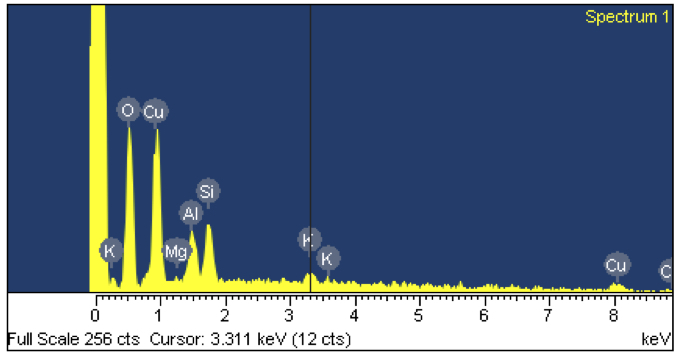
\includegraphics[width=0.8\linewidth]{HKI_nat_az_EDS_site2_spectrum1_050521_spectrumimage}
\caption[Point spectrum: HKI natural azurite]{Point spectrum: HKI natural azurite}
\label{fig:hki_eds_spectrum}
\end{figure}

\begin{figure}[H]
\centering
  \includegraphics[width=0.6\linewidth]{HKI_nat_az_EDS_site2_spectrum1_050521_semimage}
\caption[SEM image showing point spectrum sample location: HKI natural azurite]{SEM image showing point spectrum sample location: HKI natural azurite}
\label{fig:hki_eds_sem_image}
\end{figure}

\begin{table}[H]
\caption{HKI natural azurite: EDS quantitative data}
\centering
\label{table:hki_ratios}
\begin{tabular}{c c c}
\toprule
\multicolumn{3}{c}{HKI natural azurite} \\
\midrule
~ & Cu:O & Si:O \\
\midrule
\textit{Fig. \ref{fig:hki_point_eds_1}} & 0.0104 & 0.2152 \\
\textit{Fig. \ref{fig:hki_point_eds_2}} & 0.2558 & 0.0465 \\
\textit{Fig. \ref{fig:hki_point_eds_3}} & 0.0114 & 0.2906 \\
\textit{Fig. \ref{fig:hki_point_eds_4}} & 0.0040 & 0.1816 \\
\textit{Fig. \ref{fig:hki_point_eds_5}} & 0.3498 & 0.1667 \\
\textit{Fig. \ref{fig:hki_eds_spectrum}, \ref{fig:hki_eds_sem_image}} & 0.0251 & 0.3351  \\
\textit{Fig. \ref{fig:hki_point_eds_7}} & 0.0097 & 0.2499 \\
\textit{Fig. \ref{fig:hki_point_eds_8}} & 0.0060 & 0.1696 \\
\bottomrule
\end{tabular}
\end{table}

EDS mapping data is shown in \textit{Figures \ref{fig:hki_map1}}. Copper and oxygen abundance is correlated, and copper comprises approximately 50\% of the mapped area. Carbon, potassium, and magnesium distributions appear random. Iron is correlated with oxygen, suggesting iron oxide is present in low abundance. 

Silicon is generally correlated to oxygen and aluminium, though one area shows a silicon/oxygen containing compound without aluminium. There is no link between SEM morphology and elemental composition; smaller surface particles are not elementally distinct from the larger substrate. The sample consists of as much or more copper-free content as copper-containing content, and only one of eight spectra shows the expected Cu:O atomic ratio. 

\begin{figure}[H]
\centering
  \includegraphics[width=0.9\linewidth]{HKI_nat_az_EDS_map1_050521_imgs}
\caption[EDS mapping data: HKI natural azurite]{EDS mapping data: HKI natural azurite}
\label{fig:hki_map1}
\end{figure}


% ************************************************    Az1    ********************************************************************

C, O, Cu, Al, and Si were detected in Az1. \textit{Table \ref{table:az1_ratios}} shows Cu:O atomic ratios. The average Cu:O ratio value is 0.3031 (SD = 0.0631). This is on the lower end of expected ratio values for azurite, though several individual values match that expected. The Si:O ratios consistently average 0.04, and Si:Al ratios are also consistent, averaging 1.44, though silicon was not present in all spectra.

\begin{table}[H]
\caption{Az1: EDS quantitative data}
\centering
\label{table:az1_ratios}
\begin{tabular}{c c}
\toprule
\multicolumn{2}{c} {Az1, azurite} \\
\midrule
~ & Cu:O \\
\midrule
\textit{Fig. \ref{fig:az1_point_eds_1}} & 0.3150 \\
\textit{Fig. \ref{fig:az1_point_eds_2}} & 0.3236 \\
\textit{Fig. \ref{fig:az1_point_eds_3}} & 0.2920 \\
\textit{Fig. \ref{fig:az1_point_eds_4}} & 0.2018 \\
\textit{Fig. \ref{fig:az1_point_eds_5}} & 0.3969 \\
\textit{Fig. \ref{fig:az1_point_eds_6}} & 0.2893 \\
\bottomrule
\end{tabular}
\end{table}

\textit{Figure \ref{fig:az1_map1}} shows mapping data for Az1. Copper and oxygen are correlated. Detection of zinc occurs in the same areas of the sample as copper, and as these two elements have closely overlapping peaks, this attribution is interpreted as in error. Silicon and aluminium appear concurrently in smaller areas, suggesting that an aluminosilicate is present in association. Silicon also appears independent of aluminium, strongly correlated with oxygen, which suggests quartz. 

\begin{figure}[H]
\centering
  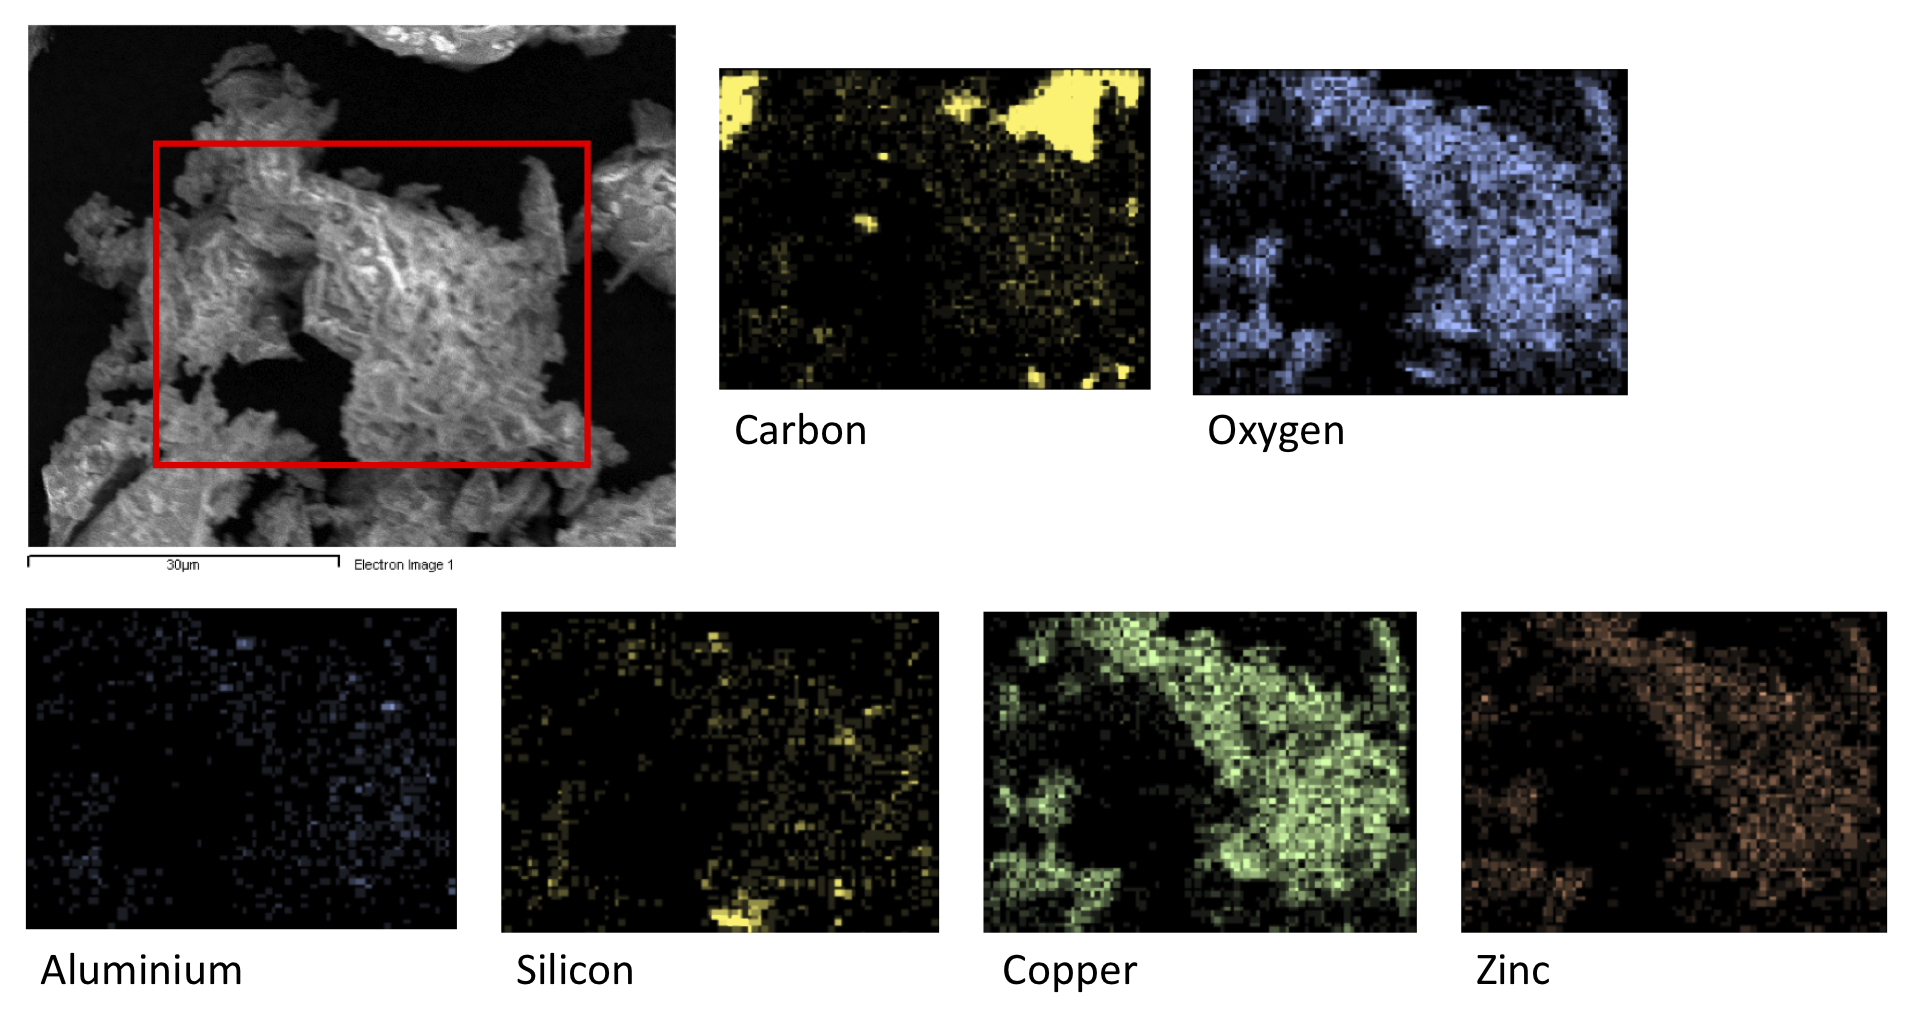
\includegraphics[width=0.9\linewidth]{Az1_EDS_map2_250221_img}
\caption[EDS mapping data: Az1]{EDS mapping data: Az1}
\label{fig:az1_map1}
\end{figure}


% ************************************************    Az2    ********************************************************************

C, O, Cu, and Si were detected in Az2. Cu:O ratios are inconsistent, 0.2699 and 0.3897 (\textit{Table \ref{table:az2_ratios}}). However, the calculated Si:O ratios at the same locations do not explain the fluctuation; the ratio of 0.0198 Si:O is far too small to indicate a silicon oxide type mineral.

\begin{table}[H]
\caption{Az2: EDS quantitative data}
\centering
\label{table:az2_ratios}
\begin{tabular}{c c c}
\toprule
\multicolumn{3}{c}{Az2, azurite} \\
\midrule
~ & Cu:O & Si:O \\
\midrule
\textit{Fig. \ref{fig:az2_point_eds_1}} & 0.2699 & 0.0198 \\
\textit{Fig. \ref{fig:az2_point_eds_2}} & 0.3897 & 0 \\
\bottomrule
\end{tabular}
\end{table}

\textit{Figure \ref{fig:az2_map1}} shows that while copper and oxygen are highly correlated, silicon and carbon are randomly distributed. This suggests that silicon is present as a trace rather than a major component, supported by low Si:O ratios. The variation in Cu:O atomic ratios must be due to a factor other than intensity due to another detectable mineral.

\begin{figure}[H]
\centering
  \includegraphics[width=0.9\linewidth]{Az2_EDS_map1_250221_img}
\caption[EDS mapping data: Az2]{EDS mapping data: Az2}
\label{fig:az2_map1}
\end{figure}

% ************************************************    AzMag    ********************************************************************

C, O, Cu, Si, and Ca are detected in AzMag. Cu:O ratios, shown in \textit{Table \ref{table:azmag_ratios}}, are 0.1786 and 0.3404. These are inconsistent: 0.3404 is very close to the expected ratio, but 0.1786 is well outside. Silicon is present at very low levels (approximate Si:O ratio = 0.01), and does not explain this variation. Calcium is present in the first sample with a ratio of 0.1012, which is significant. It is possible that a calcium containing mineral is present throughout this sample, a conclusion surprisngly not supported by mapping data.

\begin{table}[H]
\caption{AzMag: EDS quantitative data}
\centering
\label{table:azmag_ratios}
\begin{tabular}{c c}
\toprule
\multicolumn{2}{c} {AzMag, azurite} \\
\midrule
~ & Cu:O \\
\midrule
\textit{Fig. \ref{fig:azmag_point_eds_1}} & 0.1786 \\
\textit{Fig. \ref{fig:azmag_point_eds_1}} & 0.3404 \\
\bottomrule
\end{tabular}
\end{table}

\textit{Figure \ref{fig:azmag_map1}} shows mapping data for sample AzMag. Silicon and carbon show lower intensity than copper and oxygen, but all four are closely spatially correlated. Calcium was not detected in mapping data.

\begin{figure}[H]
\centering
  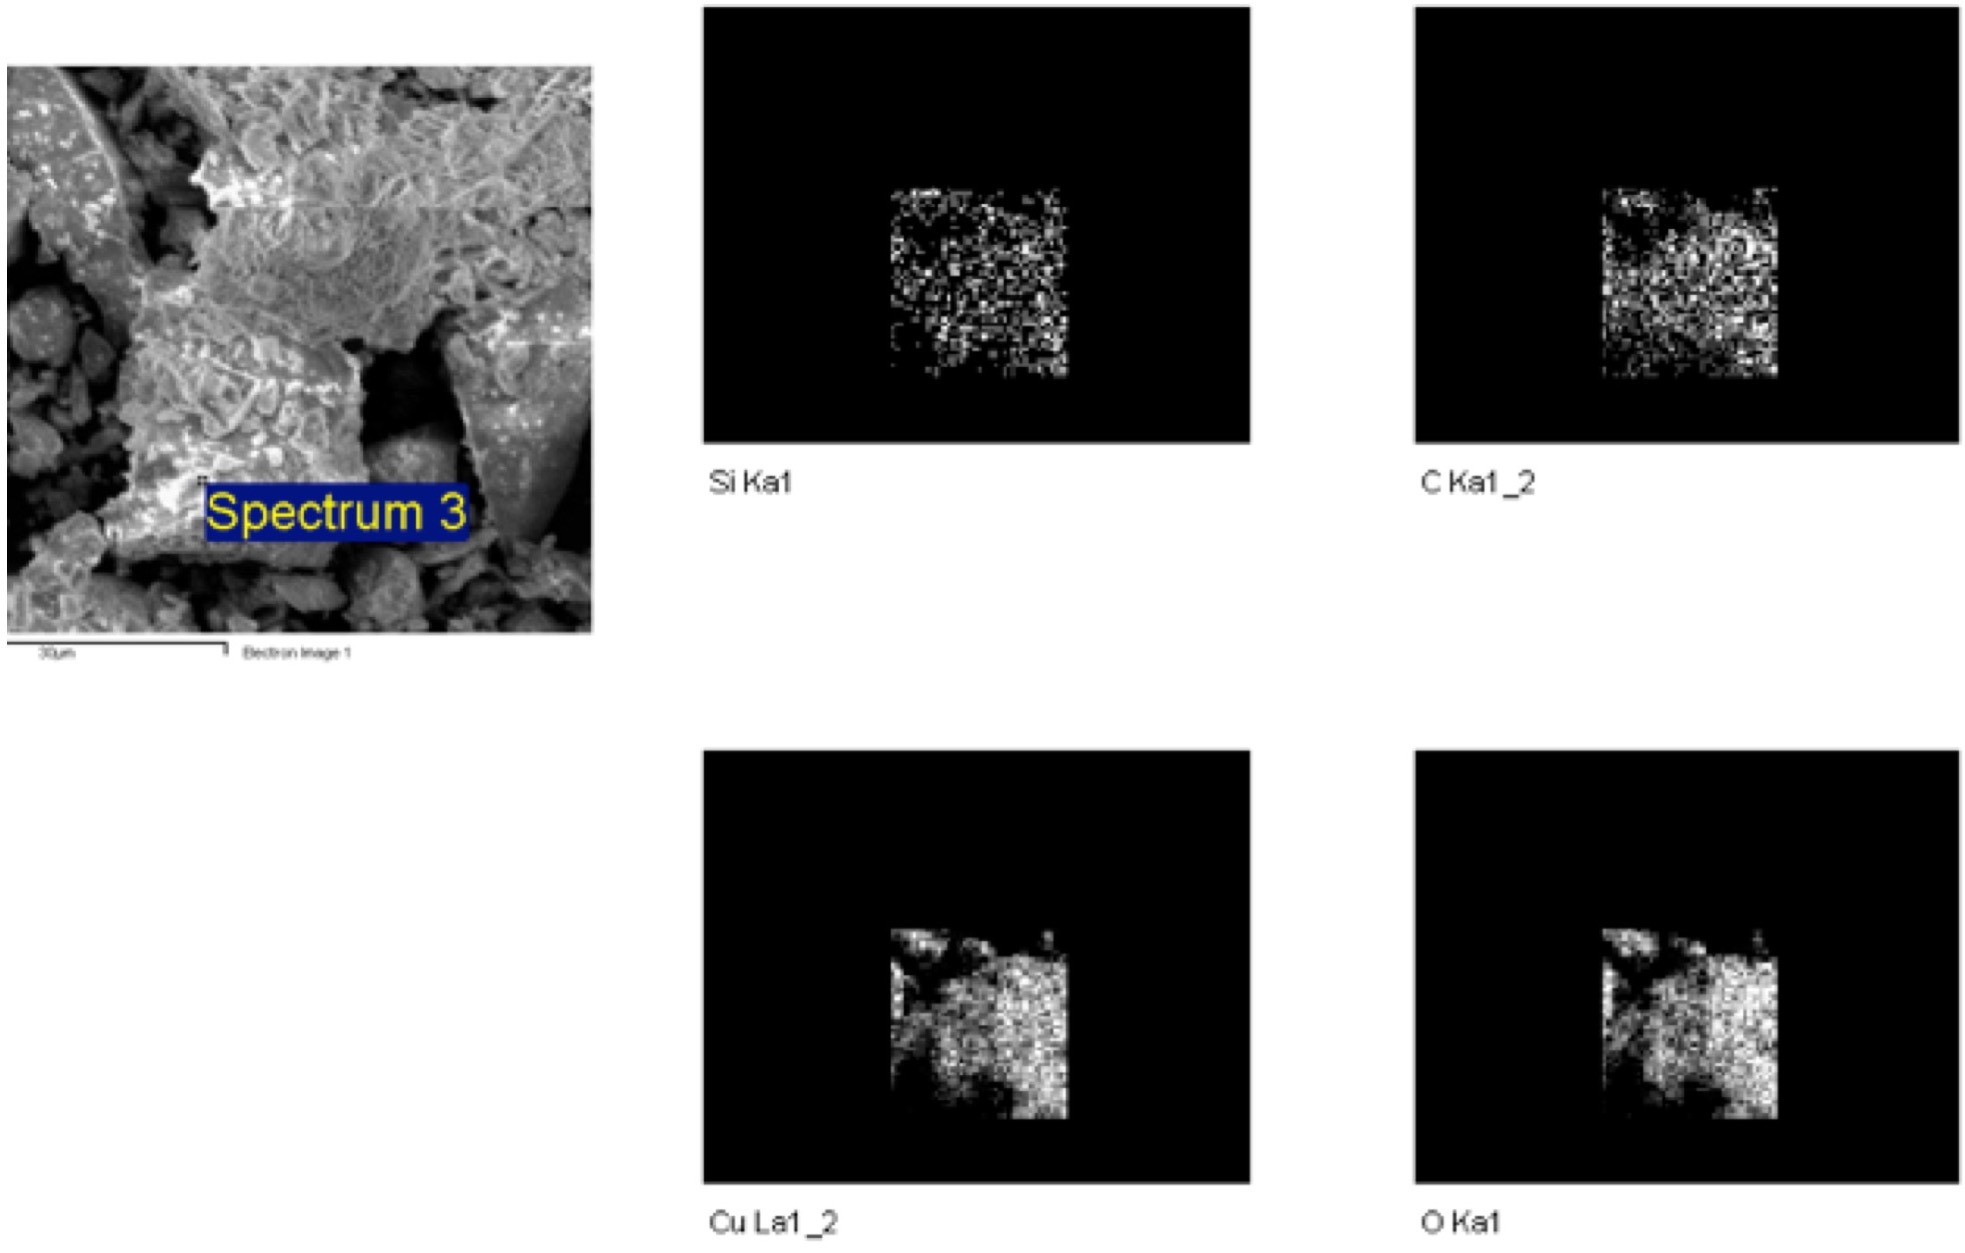
\includegraphics[width=0.9\linewidth]{AzMag_EDS_map1_260221_imgs}
\caption[EDS mapping data: AzMag]{EDS mapping data: AzMag}
\label{fig:azmag_map1}
\end{figure}


% ************************************************    AzOp    ********************************************************************

C, O, Cu, Al, and Si are detected in sample AzOp. Atomic ratios are presented in \textit{Table \ref{table:azop_ratios}}. Cu:O ratios are very low while those of Si:Al and Si:O are relatively high compared to other samples. This suggests that AzOp contains minerals such as quartz or aluminosilicates, though the experimental atomic ratios do not fit empirical formulae.

\begin{table}[H]
\caption{AzOp: EDS quantitative data}
\centering
\label{table:azop_ratios}
\begin{tabular}{c c c c}
\toprule
\multicolumn{4}{c}{AzOp, azurite} \\
\midrule
~ & Cu:O & Si:Al & Si:O \\
\midrule
\textit{Fig. \ref{fig:azop_point_eds_1}} & 0.2330 & 1.2572 & 0.1051 \\
\textit{Fig. \ref{fig:azop_point_eds_1}} & 0.2062 & 1.1140 & 0.0753 \\
\bottomrule
\end{tabular}
\end{table}

\textit{Figure \ref{fig:azop_map1}} shows mapping data for AzOp. Copper and oxygen are clearly correlated, and carbon is somewhat correlated to copper and oxygen; expected for a basic copper carbonate. Significant correlation between silicon and oxygen is also observed. Silicon is abundant across AzOp. Surprisingly, aluminium is not observed. 

\begin{figure}[H]
\centering
  \includegraphics[width=0.9\linewidth]{AzOp_EDS_map1_260221_imgs}
\caption[EDS mapping data: AzOp]{EDS mapping data: AzOp}
\label{fig:azop_map1}
\end{figure}

% ************************************************    Fitz1    ********************************************************************

C, O, Cu, Al (mapping only), Si, and Ca are detected in Fitz1. Atomic ratios are shown in \textit{Table \ref{table:fitz1_ratios}}. As Fitz1 is a synthetic pigment, it is reasonable to hypothesize that it would contain only carbon, copper, and oxygen and show consistent Cu:O ratios across point spectra. Surprisingly, low levels of silicon and calcium are detected, and Cu:O ratios range from 0.1366 (well below expected) to 0.3314. Furthermore, the chemical variation is interesting in contrast to the morphological consistency.

\begin{table}[H]
\caption{Fitz1: EDS quantitative data}
\centering
\label{table:fitz1_ratios}
\begin{tabular}{c c c c}
\toprule
\multicolumn{4}{c}{Fitz1, blue verditer} \\
\midrule
~ & Cu:O & Ca:O & Si:O \\
\midrule
\textit{Fig. \ref{fig:fitz1_point_eds_1}} & 0.2316 & 0.1555 & 0 \\
\textit{Fig. \ref{fig:fitz1_point_eds_2}} & 0.3115 & 0 & 0.0122 \\
\textit{Fig. \ref{fig:fitz1_point_eds_3}} & 0.1366 & 0.2510 & 0 \\
\textit{Fig. \ref{fig:fitz1_point_eds_4}} & 0.3314 & 0 & 0.0085 \\
\bottomrule
\end{tabular}
\end{table}

\textit{Figure \ref{fig:fitz1_map1}} shows mapping data for Fitz1. Copper is spatially correlated with some areas of oxygen, as is carbon. Calcium appears randomly distributed, and its detection is tentative because instrument noise would produce this type of spatial distribution as well. Silicon correlates to oxygen in several areas of high intensity, and aluminium and silicon are also correlated.

\begin{figure}[H]
\centering
  \includegraphics[width=0.9\linewidth]{Fitz1_EDS_map1_030321_imgs}
\caption[EDS mapping data: Fitz1]{EDS mapping data: Fitz1}
\label{fig:fitz1_map1}
\end{figure}

% ************************************************    KE3    ********************************************************************

C, O, Cu, Ca, and Si (mapping only) are detected in KE3. \textit{Table \ref{table:ke3_ratios}} shows Cu:O and Ca:O ratios. While the first Cu:O ratio is expected, the second is lower, outside the expected range. This correlates with a much larger Ca:O ratio, suggesting that calcium carbonate rather than copper carbonate is present in some sample areas. Calcium carbonate appears calcite in chalk and is a reasonable compound to detect in these samples.

\begin{table}[H]
\caption{KE3: EDS quantitative data}
\centering
\label{table:ke3_ratios}
\begin{tabular}{c c c}
\toprule
\multicolumn{3}{c}{KE3, light verditer bice} \\
\midrule
~ & Cu:O & Ca:O \\
\midrule
\textit{Fig. \ref{fig:ke3_point_eds_1}} & 0.3411 & 0.0069 \\
\textit{Fig. \ref{fig:ke3_point_eds_2}} & 0.2052 & 0.1108 \\
\bottomrule
\end{tabular}
\end{table}

\textit{Figure \ref{fig:ke3_map1}} shows mapping data for KE3. Silicon appears in mapping data sporadically but not in point spectra. Copper is correlated with oxygen, as is calcium.

\begin{figure}[H]
\centering
  \includegraphics[width=0.9\linewidth]{KE3_EDS_map1_050321_imgs}
\caption[EDS mapping data: KE3]{EDS mapping data: KE3}
\label{fig:ke3_map1}
\end{figure}

% ************************************************    KE4    ********************************************************************

C, O, Cu, and Ca were detected in KE4. Point spectra show Cu:O ratios (\textit{Table \ref{table:ke4_ratios}}) that, while slightly low, are within range of that expected for azurite (particularly the second ratio, 0.3381). Ca:O ratios are very low.

\begin{table}[H]
\caption{KE4: EDS quantitative data}
\centering
\label{table:ke4_ratios}
\begin{tabular}{c c c}
\toprule
\multicolumn{3}{c}{KE4, blue bice} \\
\midrule
~ & Cu:O & Ca:O \\
\midrule
\textit{Fig. \ref{fig:ke4_point_eds_1}} & 0.2703 & 0.0660 \\
\textit{Fig. \ref{fig:ke4_point_eds_2}} & 0.3381 & 0.0095 \\
\bottomrule
\end{tabular}
\end{table}

\textit{Figure \ref{fig:ke4_map1}} shows mapping data for KE4. Copper, oxygen, and carbon are spatially correlated. Calcium is correlated to oxygen in areas absent of copper, suggesting calcite may be present.

\begin{figure}[H]
\centering
  \includegraphics[width=0.9\linewidth]{KE4_EDS_map1_030321_imgs}
\caption[EDS mapping data: KE4]{EDS mapping data: KE4}
\label{fig:ke4_map1}
\end{figure}

% ************************************************    KE5    ********************************************************************

C, O, and Cu are detected in KE5. The average Cu:O ratio is 0.3150 (standard deviation = 0.0311), and all atomic ratios are shown in \textit{Table \ref{table:ke5_ratios}}. While this value is lower than expected, it is within reason given the possible error in quantitative determination of oxygen.

\begin{table}[H]
\caption{KE5: EDS quantitative data}
\centering
\label{table:ke5_ratios}
\begin{tabular}{c c}
\toprule
\multicolumn{2}{c} {KE5, blue verditer} \\
\midrule
~ & Cu:O \\
\midrule
\textit{Fig. \ref{fig:ke5_point_eds_1}} & 0.3371 \\
\textit{Fig. \ref{fig:ke5_point_eds_2}} & 0.3284 \\
\textit{Fig. \ref{fig:ke5_point_eds_3}} & 0.2794 \\
\bottomrule
\end{tabular}
\end{table}

% ************************************************    Ma1    ********************************************************************

Ma1 contains C, O, and Cu. \textit{Figure \ref{fig:ma1_map1}} shows mapping data for Ma1. Zinc appears at low abundance in mapping data, though as it is detected in the same areas as copper this is likely a misattribution due to peak overlap. Carbon, oxygen, and copper correlate, and the Cu:O ratio is 0.3675 (\textit{Fig. \ref{fig:ma1_point_eds_1}}). 

\begin{figure}[H]
\centering
  \includegraphics[width=0.9\linewidth]{Ma1_EDS_map1_250221_imgs}
\caption[EDS mapping data: Ma1]{EDS mapping data: Ma1}
\label{fig:ma1_map1}
\end{figure}

% ************************************************    KE1a    ********************************************************************

C, O, Cu, and Ca were detected in KE1a. Calcium is present in low levels, and is likely a trace element rather than a major component of the sample. The measured Cu:O ratios (\textit{Table \ref{table:ke1a_ratios}}) are within the range expected.

\begin{table}[H]
\caption{KE1a: EDS quantitative data}
\centering
\label{table:ke1a_ratios}
\begin{tabular}{c c c}
\toprule
\multicolumn{3}{c}{KE1a, green bice} \\
\midrule
~ & Cu:O & Ca:O \\
\midrule
\textit{Fig. \ref{fig:ke1a_point_eds_1}} & 0.3483 & 0.0086 \\
\textit{Fig. \ref{fig:ke1a_point_eds_2}} & 0.3622 & 0.0066 \\
\bottomrule
\end{tabular}
\end{table}

% ************************************************    KE2    ********************************************************************

C, O, Cu, and Si (mapping only) were detected in KE2. The measured Cu:O ratios (\textit{Table \ref{table:ke2_ratios}} are within the range expected, and are among the highest measured of any samples.

\begin{table}[H]
\caption{KE2: EDS quantitative data}
\centering
\label{table:ke2_ratios}
\begin{tabular}{c c}
\toprule
\multicolumn{2}{c} {KE2, green verditer} \\
\midrule
~ & Cu:O \\
\midrule
\textit{Fig. \ref{fig:ke2_point_eds_1}} & 0.3724 \\
\textit{Fig. \ref{fig:ke2_point_eds_2}} & 0.3944 \\
\bottomrule
\end{tabular}
\end{table}

\textit{Figure \ref{fig:ke2_map1}} shows mapping data for KE2. Carbon is sparsely distributed, and there are areas without any elements detected. Silicon, which is not detected in point spectra, is present in low levels. Copper and oxygen are highly correlated.

\begin{figure}[H]
\centering
  \includegraphics[width=0.9\linewidth]{KE2_ES_map1_040321_imgs}
\caption[EDS mapping data: KE2]{EDS mapping data: KE2}
\label{fig:ke2_map1}
\end{figure}


All green samples (Ma1, KE1a, and KE2) show Cu:O atomic ratios that closely match the expected ratios for azurite and malachite. The chemical formula for green verditer is uncertain, and the margin of error on quantitative analysis is not able to distinguish between a 2:5 and a 3:8 Cu:O ratio. Associate minerals are minimally present in these samples, and their Cu:O ratios confirm basic copper carbonates.

%       *****************************

Mapping data for the cross section collected on the JEOL and TESCAN SEM-EDS instruments are presented in \textit{Figures \ref{fig:xsection_map1}} and \textit{Figure \ref{fig:xsection_map2}}. The cross section consists of three visually distinct layers, but EDS mapping data shows that layers A and B (in \textit{Figure \ref{fig:hki_crossec_explanation}}) are chemically comparable. The visual difference is due to the higher concentration of lead containing components in layer B. 

Oxygen is distributed across the entire sample, which is expected as many common pigments carbonates or oxides and organic binder components also contain oxygen. Calcium, aluminium, and silicon are detected over the entire sample, with correlation between aluminium and silicon. It is likely that an aluminosilicate is present as an associate mineral. Calcium-based ground layers are common, and a material like limestone could contain calcium, silicon, aluminium, and potassium, also detected in the cross section. Potassium is observed in HKI natural azurite, suggesting it is a hallmark of azurite samples.

Aluminosilicates are present as distinct components, as observed in \textit{Figure \ref{fig:xsection_map2}} where silicon and aluminium are precisely localised. Calcite, a common mineral associated with azurite, is observed in most powder samples, natural and artificial. Calcium carbonates and aluminosilicates were also commonly used as paint extenders, white particles mixed with coloured pigments to lower their cost to produce.~\autocite{Townsend}

Magnesium, lead, and copper are localised to areas of the sample corresponding to distinct pigment particles or aggregates. The lead pigment present is likely lead white, a basic lead(II) carbonate occurring as a mineral called cerussite. While cerussite may occur in association with natural azurite, the abundance of lead and the lack of overlapping areas of lead and copper suggests that lead white was employed as a pigment mixed with the blue azurite.~\autocite{Aru}

Magnesium oxides are historical pigments, most importantly \textit{terre verte}, a green mixture of an iron silicate with a magnesium-containing clay. Low iron abundance discourages the assignment of magnesium to terre verte; magnesium-based minerals associated with azurite or cerussite are likelier. Magnesium may be present as mica or another common mineral. Iron is detected sporadically, suggesting that it is a trace element. Arsenic is suggested in one EDS map (\textit{Figure \ref{fig:xsection_map2}}), commonly associated with lead in nature. \textit{Figure \ref{fig:xsection_map2}} shows mapping data collected from the TESCAN SEM at approximately 2000x magnification. In addition to detecting arsenic, this map confirms the results acquired on the JEOL instrument.

Copper containing areas show a Cu:O ratio of, on average, 0.217. This is lower than the expected. Also detected in these areas are high levels of iron and lead, indicating impurities in the blue pigment particles (iron) and/or contribution from the three dimensional structure of the paint mixture containing azurite and lead white. Silicon and magnesium are detected at lower levels and both make up common associate minerals of azurite.

This data demonstrates the complexity of analysis of samples consisting of a mixture of different pigments, each containing various associate minerals.

%O, Cu, Ca, Pb, Mg, Al, Si, K, Fe ( map only: As??)

%Darkest: Mg on mapping (low atomic number)
%Lightest: Lead, fine powder, widely distributed through one of the laters, likely mixed with Cu to make a lighter color (lead white)
%Moderate: Copper
%Darker layer shows relatively more Si in mapping

\begin{figure}[H]
\centering
  \includegraphics[width=0.9\linewidth]{hki_cross_section_eds_analysis_250621_site1_map1}
\caption[EDS mapping data: cross section, JEOL SEM]{EDS mapping data: cross section, JEOL SEM}
\label{fig:xsection_map1}
\end{figure}

\begin{figure}[H]
\centering
  \includegraphics[width=0.98\linewidth]{HKI_cross_section_Site 7_2021-06-30_15-23-55}
\caption[EDS mapping data: cross section, TESCAN SEM]{EDS mapping data: cross section, TESCAN SEM}
\label{fig:xsection_map2}
\end{figure}

\subsection[Summary of EDS results]{Summary of EDS results}

\textit{Table \ref{table:eds_data_summary}} summarizes detected elements and average Cu:O ratios for copper-containing point spectra collected from each reference sample. Natural azurite samples showed greater diversity of elements than synthetic samples. Most samples including verditers contained calcium, suggesting that may result from the industrial synthetic process. Cu:O ratios, on the other hand, were not diagnostic for sample origin, consistent across all samples within error. For sample Fitz1, two Cu:O ratios are presented as several points sampled showed large Ca:O ratios that led to a low Cu:O average. The larger Cu:O ratio excludes these points.

\begin{table}[H]
\caption{Summary of EDS data results: reference samples}
\centering
\label{table:eds_data_summary}
\begin{tabular}{c c c}
\toprule
Sample & Detected elements & Cu:O ratio $\pm$ SD \\
\midrule
HKI natural azurite & C, O, Cu, Si, Al, Mg, Ca, K, Fe & 0.3028 $\pm$ 0.0664 \\
Az1 & C, O, Cu, Si, Al & 0.3031 $\pm$ 0.0631 \\
Az2 & C, O, Cu, Si & 0.3298 $\pm$ 0.0847 \\
AzMag & C, O, Cu, Si, Ca & 0.2595 $\pm$ 0.1144 \\
AzOp & C, O, Cu, Si, Al  & 0.2196 $\pm$ 0.0190 \\
Fitz1 & C, O, Cu, Si, Ca & \vtop{\hbox{\strut 0.2528 $\pm$ 0.0886}\hbox{\strut 0.3215 $\pm$ 0.0141}} \\    
KE3 & C, O, Cu, Ca & 0.2732 $\pm$ 0.0961 \\
KE4 & C, O, Cu, Ca & 0.3042 $\pm$ 0.0479 \\
KE5 & C, O, Cu & 0.3150 $\pm$ 0.0311 \\
Ma1 & C, O, Cu & \textemdash \\
KE1a & C, O, Cu, Ca & 0.3553 $\pm$ 0.0098 \\
KE2 & C, O, Cu & 0.3834 $\pm$ 0.0156 \\
Cross section & C, O, Cu, Si, Al, Mg, Ca, K, Fe, Pb, As & \textemdash \\
\bottomrule
\end{tabular}
\end{table}



% *******************************************************************************************************************************
% *******************************************************************************************************************************
% *******************************************************************************************************************************

\section[Raman Data]{Raman Data}
\label{section3.3}

\textit{Figure \ref{fig:label_raman}} shows Raman spectra of samples Az1 (blue) and Ma1 (green). The spectrum from Az1 was collected from a bright blue particle, while the spectrum from Ma1 was collected from fine green bulk particles. Both therefore are representative of the component of the pigment responsible for the colour rather than of an impurity.

Hydroxyl stretching bands were reported by Frost et. al. for azurite at 3453 and 3427 cm\textsuperscript{-1} and for malachite at 3468 and 3386 cm\textsuperscript{-1}.~\autocite{Frost} These bands are not shown here. Mattei et. al. assign bands below 600 cm\textsuperscript{-1} to CuO vibrations and bands from 600 to 1600 cm\textsuperscript{-1} to carbonate vibrations.~\autocite{Mattei}

The Raman spectra shown in \textit{Figure \ref{fig:label_raman}} agree closely with literature peak locations.~\autocite{Mattei,Frost,Bicchieri} The technique is capable of identifying azurite and malachite (or their synthetic analogues).

\begin{comment}
azurite
Frost: $v1    v2_Sym  v2_Antisym   v3_B2   v3_A1    v4_B2   v4_A1$
       1095   816       834        1419    1430     765     739

Bicchieri: 145, 180, 250, 284, 335, 403, 545, 746, 767, 839, 940, 1098, 1432 and 1573 cm

Mattei: 157vw 174vw 182vw 240vw 250vw \textbf{267vw} 282vw 332vw
\textbf{387vw} 402s 542vw \textbf{744vw is shoulder} 768w 840w 937vw 1099m
1422m(sh) \textbf{1433m is shoulder in mine} 1462vw 1582w 3431w

Me: 113 139 180 248 284 330 401 507 541 577 764 836 937 1096 1419 1459 1576


malachite

mattei: \textbf{157m(sh) 171m(sh) 182s 204vw 224vw} 272s 352w 435s 513w
537m 601vw 723vw 753vw 1058w 1101w 1370vw 1463vw
1497s 3380w

frost: $v1    v2_Sym  v2_Antisym   v3_B2   v3_A1    v4_B2   v4_A1$
      1096     816      801       1492     1364     752     717
                                  1514     1423

Me: 120 144 153 168 180 222 269 352 433 509 533 565 598 720 749
\end{comment}

Spectra comparing reference azurite and verditer pigments are shown in \textit{Figure \ref{fig:blue_comparison1}}-\textit{\ref{fig:blue_comparison3}}. All spectra were collected from bulk particles. The Raman spectra of natural samples are compared in \textit{Figure \ref{fig:blue_comparison1}} and \textit{Figure \ref{fig:blue_comparison2}} (alongside KE4, of ambiguous origin). The Raman spectra of synthetic samples are compared in \textit{Figure \ref{fig:blue_comparison3}}. All green samples are compared in \textit{Figure \ref{fig:green_comparison}}.

Natural azurite samples show consistent peak locations, though intensity ratios vary. Samples Fitz1, KE3, KE4, and KE5 are also consistent. The low frequency region shows variation between natural and synthetic samples. This is the lattice vibration region, and variation suggests that bond structures differ in crystals depending on origin. Frost et. al. showed that the band intensities of azurite depend on crystal orientation and polarisation, so the differences in band intensities are expected and not used to distinguish between different chemistries.~\autocite{Frost}

Green samples varied in the region of 400-600 cm\textsuperscript{-1}, showing a strong peak at either 400 cm\textsuperscript{-1} and 450 cm\textsuperscript{-1} or 430 cm\textsuperscript{-1}. The natural malachite sample Ma1 also shows additional bands above 500 cm\textsuperscript{-1} that are not clearly observed in the rest. 

These results suggest that although interpretation of mineral Raman spectra is difficult due to the influence of structural variation on spectral bands, this analysis may be used alongside other methods to assign the origin of a sample. Due to the variability in band intensity, especially in the lower frequency region, conclusions should not be drawn from Raman results alone.

\begin{figure}[H]
\centering
\begin{minipage}[t]{\linewidth}
  \centering
  \includegraphics[width=0.9\linewidth]{az1_blue_withlabels}
\hfill
\includegraphics[width=0.9\linewidth]{natural_malachite_graph_labelled}
\hfill
\end{minipage}
\caption[Raman spectra of natural azurite and malachite, peak centres labelled.]{Raman spectra of natural azurite (blue, top) and malachite (green, bottom). Peak centres are labelled.}
\label{fig:label_raman}
\end{figure}

\begin{figure}[H]
\centering
  \includegraphics[width=0.8\linewidth]{hki_az1_az2}
\caption[Raman spectra of blue samples.]{Raman spectra of verditer and azurite samples: HKI natural azurite, Az1, Az2. Spectra are offset for clarity.}
\label{fig:blue_comparison1}
\end{figure}

\begin{figure}[H]
  \centering
  \includegraphics[width=0.8\linewidth]{hki_azmag_azop_ke4}
\caption[Raman spectra of blue samples.]{Raman spectra of verditer and azurite samples: HKI natural azurite, AzMag, AzOp, KE4. Spectra are offset for clarity.}
\label{fig:blue_comparison2}
\end{figure}

\begin{figure}[H]
  \centering
  \includegraphics[width=0.8\linewidth]{fitz1_ke3_ke4_ke5}
\caption[Raman spectra of blue samples.]{Raman spectra of verditer and azurite samples: Fitz1, KE3, KE4, KE5. Spectra are offset for clarity.}
\label{fig:blue_comparison3}
\end{figure}

\begin{figure}[H]
\centering
  \includegraphics[width=0.8\linewidth]{ma1_ke1a_ke1b_ke2}
\caption[Raman spectra of green samples.]{Raman spectra of natural malachite and synthetic green verditer samples: Ma1, KE1a, KE1b, and KE2. Spectra are offset for clarity.}
\label{fig:green_comparison}
\end{figure}

Several powdered azurite and verditer samples contained particles that differed in colour from the main component. \textit{Figure \ref{fig:inclusion_raman}} shows green and white inclusions in samples Az2, AzMag, AzOp, KE4, and KE5. Several of these spectra are attributable to associate minerals, such as quartz and terre verte (a general term for iron-based green clays, often containing potassium, magnesium, aluminium, and silicon).~\autocite{ucl_database,cameo_mfa,irug_quartz} Quartz and various clays are expected based on known associate minerals.

Two green inclusions in blue samples show strong bands that correlate to azurite and malachite. Malachite is a common associate of azurite, as well as a degradation product. From the historical record of verditer production, it is known that crystals vary in colour from blue to green depending upon environmental conditions, and this may also explain the green colour of a particle that appears to be azurite in sample AzMag. It is reasonable to think that natural samples may show colour variations. 

Two white inclusions, in samples Az2 and AzOp, are not conclusively identified. The confocal illumination system may make samples appear white if they are highly reflecting, though common metallic minerals have been excluded. The strong bands at 373, 823, and 878 cm\textsuperscript{-1} in the spectrum collected from Az2 are suggestive of Al-O and Si-O vibrational modes in aluminosilicates. Grossular garnet shows a close match to this spectrum, and has been tentatively assigned.~\autocite{Culka} One challenge present in identifying these associate minerals is that their damage threshold is often lower than that of azurite or malachite, requiring lower laser powers and shorter acquisition times.

\begin{figure}[H]
\centering
\begin{minipage}[t]{\linewidth}
  \centering
  \includegraphics[width=0.9\linewidth]{green_inclusions}
\hfill
\includegraphics[width=0.9\linewidth]{white_inclusions}
\hfill
\end{minipage}
\caption[Raman spectra of green and white mineral inclusions in azurite.]{Raman spectra of green (top) and white (bottom) mineral inclusions in azurite. Reference azurite and malachite spectra are shown for comparison purposes, and spectra are scaled and offset for clarity. Identifiable spectra are labelled, and bands attributable to copper carbonate and malachite are highlighted for ease of comparison to references.}
\label{fig:inclusion_raman}
\end{figure}

Analysis of resin embedded samples (e.g. cross sections), proved difficult using the confocal Raman system. \textit{Figure \ref{fig:fluor_example_graph}} shows spectra collected using an excitation wavelength of 532 nm from the surface of the cross section. Azurite is clearly present in one spectrum (black) with a strong band at 400 cm\textsuperscript{-1} (highlighted in blue). Cerussite (lead white) is present in both spectra (highlighted in grey). Broad baselines were subtracted but based on presence of interference fringing, additional fluorescence is present. Analysis of the polyester resin without pigment shows that these bands are from resin.

These bands are present in all spectra collected from cross sections. The signal is strong enough to mask contributions from azurite and is comparable in intensity to contributions from cerussite, a major component of the cross section along with azurite. This clearly poses a problem for detection of variation in pigments and introduces uncertainty.

\textit{Figure \ref{fig:contours_xsection}} shows contour plots of azurite peak intensity (left) and integrated peak area (right) across a 10 x 10 spectrum map of an area of the cross section. The uncertainty introduced by resin bands is apparent, as peak area and peak intensity do not indicate azurite particles are present in the same areas of the map. This is due to varying contributions from the underlying fluorescence band that are difficult to subtract without introducing additional errors into the analysis.

\begin{figure}[H]
\centering
  \includegraphics[width=0.9\linewidth]{fluor_example_graph}
\caption[Raman spectra of cross section]{Raman spectra of two points on cross section, blue area. The interference fringing observed is due to fluorescence from the resin (contribution from non-azurite pigment particles and organic binder is also possible). The major azurite (blue) and cerussite (grey) peaks are highlighted on the graph and spectra are offset for clarity.}
\label{fig:fluor_example_graph}
\end{figure}


\begin{figure}[H]
\centering
\begin{minipage}{.45\textwidth}
  \centering
  \includegraphics[width=\linewidth]{050721map400intensities}
\end{minipage}
\begin{minipage}{.45\textwidth}
  \centering
  \includegraphics[width=\linewidth]{050721map400areas}
\end{minipage}
\caption[Contour maps, azurite Raman intensity in cross section]{Contour maps show the Raman intensity as: \textbf{left)} 400 cm\textsuperscript{-1} peak intensity and \textbf{right)} 400 cm\textsuperscript{-1} integrated peak area. X and Y axes map to locations on the sample surface where spectra were collected, in total 10 x 10 = 100 spectra.}
\label{fig:contours_xsection}
\end{figure}

The 473 nm excitation wavelength was also tested to determine whether the fluorescence would be mitigated by shifting the excitation frequency. This did not resolve the issue, with fluorescence and sample bands showing a similar increase in intensity at 473 nm. It may be possible to generate sample spectra without fluorescence by moving to the anti-Stokes region where fluorescence is not possible. However, this comes at the cost of intensity and signal-to-noise strength.

%az1_blue_withlabels
%Ma1_labels

%green_pigments_all_labels
%blue_HKI_AzMag_AzOp_Ke4
%blue_HKI_Az1_Az2_labels
%blue_Fitz1_Ke5_Ke3_labels
%blue_Fitz1_Ke5_Ke3_Ke4_labels


% *******************************************************************************************************************************
% *******************************************************************************************************************************
% *******************************************************************************************************************************

\section[AFM Data]{AFM Data}
\label{section3.4}

%      HKI natural azurite

AFM images recorded in tapping mode capture height, deflection, and phase variation across the sample surface. Phase and deflection measurements record variations in mechanical and chemical properties that are not easily deconvoluted or quantified. Deflection refers to the displacement of the tip with interaction with the surface, and phase shift refers to the difference between the oscillation frequency of the tip before and after interaction.~\autocite{iscpi} Phase shift and deflection measurements are affected by changes in tip-surface interaction such as adherence or repulsion. 

Height effects can appear in phase and deflection maps as intensity changes that change direction as the tip passes over a structure on the sample surface. These look, for instance, like a high deflection voltage or phase shift on the left side of the structure and a low deflection voltage or phase shift on the right side as the tip scans left to right. This is due to changing the contact area of the tip with the sample as it approaches a change in topography.~\autocite{iscpi} 

\textit{Figure \ref{fig:afm_hki_nataz_height_phase_1}} shows height and phase shift maps of an 80 x 80 $\mu$m area of HKI natural azurite. The surface texture is very dense and shows small circular particles. Tip dragging on the surface causes distortions to the image. 

Additional AFM and AFM-IR images are presented in Appendix A, Supplemental data. Although this method has potential in the analysis of highly polished or microtomed mineral samples, preparation capability has not allowed sufficiently flat surfaces for clear imaging, leading to images with instrumental artefacts obscuring information about the sample. Deflection images showed primarily instrument artefacts. Additionally, infrared measurements on the instrument currently are not reliable. This technique may be revisited in the future.

\begin{figure}[H]
\centering
\begin{minipage}{.45\textwidth}
  \centering
  \includegraphics[width=\linewidth]{hki_nataz_tapping_mode_150721_height_1}
\end{minipage}
\begin{minipage}{.45\textwidth}
  \centering
  \includegraphics[width=\linewidth]{hki_nataz_tapping_mode_150721_phase_1}
\end{minipage}
\caption[Height and phase maps, HKI natural azurite]{Height and phase maps, HKI natural azurite, 80 x 80 $\mu$m.}
\label{fig:afm_hki_nataz_height_phase_1}
\end{figure}




